% Created by tikzDevice version 0.9 on 2016-03-14 23:41:45
% !TEX encoding = UTF-8 Unicode
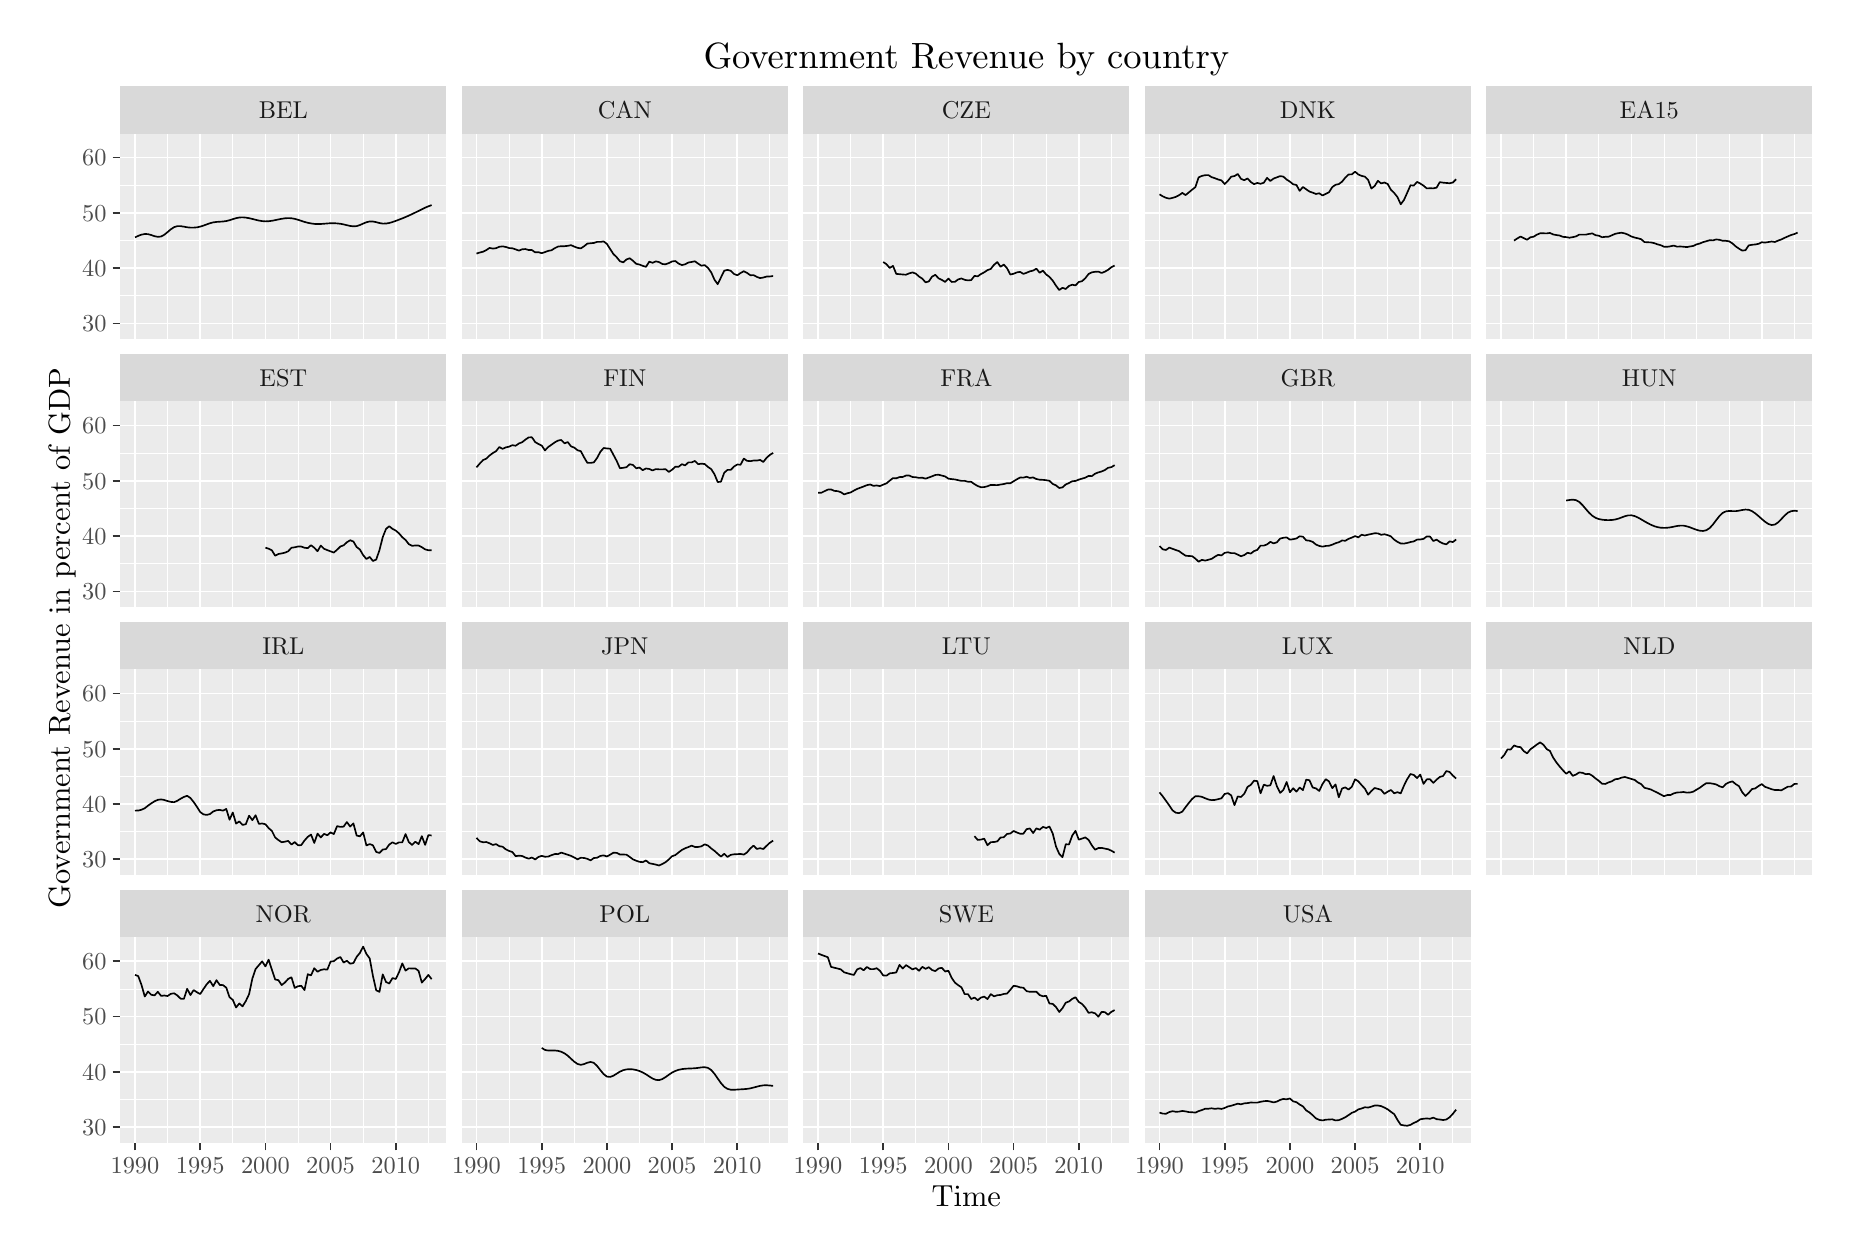
\begin{tikzpicture}[x=1pt,y=1pt]
\definecolor{fillColor}{RGB}{255,255,255}
\path[use as bounding box,fill=fillColor,fill opacity=0.00] (0,0) rectangle (650.43,433.62);
\begin{scope}
\path[clip] (  0.00,  0.00) rectangle (650.43,433.62);
\definecolor{drawColor}{RGB}{255,255,255}
\definecolor{fillColor}{RGB}{255,255,255}

\path[draw=drawColor,line width= 0.6pt,line join=round,line cap=round,fill=fillColor] (  0.00,  0.00) rectangle (650.43,433.62);
\end{scope}
\begin{scope}
\path[clip] ( 33.42,321.12) rectangle (151.33,395.37);
\definecolor{fillColor}{gray}{0.92}

\path[fill=fillColor] ( 33.42,321.12) rectangle (151.33,395.37);
\definecolor{drawColor}{RGB}{255,255,255}

\path[draw=drawColor,line width= 0.3pt,line join=round] ( 33.42,336.72) --
	(151.33,336.72);

\path[draw=drawColor,line width= 0.3pt,line join=round] ( 33.42,356.71) --
	(151.33,356.71);

\path[draw=drawColor,line width= 0.3pt,line join=round] ( 33.42,376.69) --
	(151.33,376.69);

\path[draw=drawColor,line width= 0.3pt,line join=round] ( 50.56,321.12) --
	( 50.56,395.37);

\path[draw=drawColor,line width= 0.3pt,line join=round] ( 74.12,321.12) --
	( 74.12,395.37);

\path[draw=drawColor,line width= 0.3pt,line join=round] ( 97.67,321.12) --
	( 97.67,395.37);

\path[draw=drawColor,line width= 0.3pt,line join=round] (121.23,321.12) --
	(121.23,395.37);

\path[draw=drawColor,line width= 0.3pt,line join=round] (144.79,321.12) --
	(144.79,395.37);

\path[draw=drawColor,line width= 0.6pt,line join=round] ( 33.42,326.72) --
	(151.33,326.72);

\path[draw=drawColor,line width= 0.6pt,line join=round] ( 33.42,346.71) --
	(151.33,346.71);

\path[draw=drawColor,line width= 0.6pt,line join=round] ( 33.42,366.70) --
	(151.33,366.70);

\path[draw=drawColor,line width= 0.6pt,line join=round] ( 33.42,386.69) --
	(151.33,386.69);

\path[draw=drawColor,line width= 0.6pt,line join=round] ( 38.78,321.12) --
	( 38.78,395.37);

\path[draw=drawColor,line width= 0.6pt,line join=round] ( 62.34,321.12) --
	( 62.34,395.37);

\path[draw=drawColor,line width= 0.6pt,line join=round] ( 85.90,321.12) --
	( 85.90,395.37);

\path[draw=drawColor,line width= 0.6pt,line join=round] (109.45,321.12) --
	(109.45,395.37);

\path[draw=drawColor,line width= 0.6pt,line join=round] (133.01,321.12) --
	(133.01,395.37);
\definecolor{drawColor}{RGB}{0,0,0}

\path[draw=drawColor,line width= 0.6pt,line join=round] ( 38.78,357.82) --
	( 39.96,358.40) --
	( 41.14,358.83) --
	( 42.32,359.06) --
	( 43.49,359.01) --
	( 44.67,358.68) --
	( 45.85,358.27) --
	( 47.03,358.02) --
	( 48.21,358.15) --
	( 49.38,358.79) --
	( 50.56,359.76) --
	( 51.74,360.77) --
	( 52.92,361.54) --
	( 54.09,361.89) --
	( 55.27,361.89) --
	( 56.45,361.71) --
	( 57.63,361.49) --
	( 58.81,361.36) --
	( 59.98,361.36) --
	( 61.16,361.47) --
	( 62.34,361.72) --
	( 63.52,362.10) --
	( 64.70,362.53) --
	( 65.87,362.95) --
	( 67.05,363.26) --
	( 68.23,363.42) --
	( 69.41,363.50) --
	( 70.58,363.57) --
	( 71.76,363.74) --
	( 72.94,364.04) --
	( 74.12,364.42) --
	( 75.30,364.78) --
	( 76.47,365.02) --
	( 77.65,365.08) --
	( 78.83,364.98) --
	( 80.01,364.77) --
	( 81.19,364.50) --
	( 82.36,364.20) --
	( 83.54,363.92) --
	( 84.72,363.72) --
	( 85.90,363.63) --
	( 87.07,363.68) --
	( 88.25,363.84) --
	( 89.43,364.06) --
	( 90.61,364.32) --
	( 91.79,364.55) --
	( 92.96,364.73) --
	( 94.14,364.81) --
	( 95.32,364.75) --
	( 96.50,364.53) --
	( 97.67,364.20) --
	( 98.85,363.81) --
	(100.03,363.43) --
	(101.21,363.11) --
	(102.39,362.87) --
	(103.56,362.71) --
	(104.74,362.65) --
	(105.92,362.68) --
	(107.10,362.77) --
	(108.28,362.87) --
	(109.45,362.95) --
	(110.63,362.96) --
	(111.81,362.89) --
	(112.99,362.75) --
	(114.16,362.53) --
	(115.34,362.24) --
	(116.52,361.97) --
	(117.70,361.83) --
	(118.88,361.92) --
	(120.05,362.30) --
	(121.23,362.82) --
	(122.41,363.31) --
	(123.59,363.59) --
	(124.76,363.57) --
	(125.94,363.33) --
	(127.12,363.02) --
	(128.30,362.82) --
	(129.48,362.83) --
	(130.65,363.04) --
	(131.83,363.38) --
	(133.01,363.80) --
	(134.19,364.24) --
	(135.37,364.70) --
	(136.54,365.19) --
	(137.72,365.70) --
	(138.90,366.25) --
	(140.08,366.82) --
	(141.25,367.40) --
	(142.43,367.99) --
	(143.61,368.56) --
	(144.79,369.07) --
	(145.97,369.49);
\end{scope}
\begin{scope}
\path[clip] (156.83,321.12) rectangle (274.73,395.37);
\definecolor{fillColor}{gray}{0.92}

\path[fill=fillColor] (156.83,321.12) rectangle (274.73,395.37);
\definecolor{drawColor}{RGB}{255,255,255}

\path[draw=drawColor,line width= 0.3pt,line join=round] (156.83,336.72) --
	(274.73,336.72);

\path[draw=drawColor,line width= 0.3pt,line join=round] (156.83,356.71) --
	(274.73,356.71);

\path[draw=drawColor,line width= 0.3pt,line join=round] (156.83,376.69) --
	(274.73,376.69);

\path[draw=drawColor,line width= 0.3pt,line join=round] (173.96,321.12) --
	(173.96,395.37);

\path[draw=drawColor,line width= 0.3pt,line join=round] (197.52,321.12) --
	(197.52,395.37);

\path[draw=drawColor,line width= 0.3pt,line join=round] (221.08,321.12) --
	(221.08,395.37);

\path[draw=drawColor,line width= 0.3pt,line join=round] (244.63,321.12) --
	(244.63,395.37);

\path[draw=drawColor,line width= 0.3pt,line join=round] (268.19,321.12) --
	(268.19,395.37);

\path[draw=drawColor,line width= 0.6pt,line join=round] (156.83,326.72) --
	(274.73,326.72);

\path[draw=drawColor,line width= 0.6pt,line join=round] (156.83,346.71) --
	(274.73,346.71);

\path[draw=drawColor,line width= 0.6pt,line join=round] (156.83,366.70) --
	(274.73,366.70);

\path[draw=drawColor,line width= 0.6pt,line join=round] (156.83,386.69) --
	(274.73,386.69);

\path[draw=drawColor,line width= 0.6pt,line join=round] (162.18,321.12) --
	(162.18,395.37);

\path[draw=drawColor,line width= 0.6pt,line join=round] (185.74,321.12) --
	(185.74,395.37);

\path[draw=drawColor,line width= 0.6pt,line join=round] (209.30,321.12) --
	(209.30,395.37);

\path[draw=drawColor,line width= 0.6pt,line join=round] (232.85,321.12) --
	(232.85,395.37);

\path[draw=drawColor,line width= 0.6pt,line join=round] (256.41,321.12) --
	(256.41,395.37);
\definecolor{drawColor}{RGB}{0,0,0}

\path[draw=drawColor,line width= 0.6pt,line join=round] (162.18,351.97) --
	(163.36,352.36) --
	(164.54,352.66) --
	(165.72,353.23) --
	(166.90,354.02) --
	(168.07,353.78) --
	(169.25,353.93) --
	(170.43,354.45) --
	(171.61,354.59) --
	(172.78,354.37) --
	(173.96,353.98) --
	(175.14,353.90) --
	(176.32,353.50) --
	(177.50,353.06) --
	(178.67,353.53) --
	(179.85,353.62) --
	(181.03,353.26) --
	(182.21,353.25) --
	(183.39,352.43) --
	(184.56,352.49) --
	(185.74,352.12) --
	(186.92,352.53) --
	(188.10,352.96) --
	(189.27,353.18) --
	(190.45,353.93) --
	(191.63,354.52) --
	(192.81,354.64) --
	(193.99,354.66) --
	(195.16,354.78) --
	(196.34,355.02) --
	(197.52,354.50) --
	(198.70,354.06) --
	(199.87,353.85) --
	(201.05,354.62) --
	(202.23,355.59) --
	(203.41,355.71) --
	(204.59,355.83) --
	(205.76,356.20) --
	(206.94,356.20) --
	(208.12,356.38) --
	(209.30,355.48) --
	(210.48,353.62) --
	(211.65,351.83) --
	(212.83,350.67) --
	(214.01,349.22) --
	(215.19,348.81) --
	(216.36,349.85) --
	(217.54,350.30) --
	(218.72,349.39) --
	(219.90,348.28) --
	(221.08,348.02) --
	(222.25,347.55) --
	(223.43,347.20) --
	(224.61,349.06) --
	(225.79,348.65) --
	(226.97,349.17) --
	(228.14,348.92) --
	(229.32,348.22) --
	(230.50,348.11) --
	(231.68,348.56) --
	(232.85,349.15) --
	(234.03,349.29) --
	(235.21,348.37) --
	(236.39,347.83) --
	(237.57,348.11) --
	(238.74,348.75) --
	(239.92,348.96) --
	(241.10,349.20) --
	(242.28,348.35) --
	(243.45,347.60) --
	(244.63,347.82) --
	(245.81,346.83) --
	(246.99,345.20) --
	(248.17,342.55) --
	(249.34,340.92) --
	(250.52,343.37) --
	(251.70,345.78) --
	(252.88,346.10) --
	(254.06,345.75) --
	(255.23,344.62) --
	(256.41,344.15) --
	(257.59,344.95) --
	(258.77,345.61) --
	(259.94,345.01) --
	(261.12,344.16) --
	(262.30,344.20) --
	(263.48,343.56) --
	(264.66,343.12) --
	(265.83,343.33) --
	(267.01,343.68) --
	(268.19,343.72) --
	(269.37,343.87);
\end{scope}
\begin{scope}
\path[clip] (280.23,321.12) rectangle (398.13,395.37);
\definecolor{fillColor}{gray}{0.92}

\path[fill=fillColor] (280.23,321.12) rectangle (398.13,395.37);
\definecolor{drawColor}{RGB}{255,255,255}

\path[draw=drawColor,line width= 0.3pt,line join=round] (280.23,336.72) --
	(398.13,336.72);

\path[draw=drawColor,line width= 0.3pt,line join=round] (280.23,356.71) --
	(398.13,356.71);

\path[draw=drawColor,line width= 0.3pt,line join=round] (280.23,376.69) --
	(398.13,376.69);

\path[draw=drawColor,line width= 0.3pt,line join=round] (297.36,321.12) --
	(297.36,395.37);

\path[draw=drawColor,line width= 0.3pt,line join=round] (320.92,321.12) --
	(320.92,395.37);

\path[draw=drawColor,line width= 0.3pt,line join=round] (344.48,321.12) --
	(344.48,395.37);

\path[draw=drawColor,line width= 0.3pt,line join=round] (368.03,321.12) --
	(368.03,395.37);

\path[draw=drawColor,line width= 0.3pt,line join=round] (391.59,321.12) --
	(391.59,395.37);

\path[draw=drawColor,line width= 0.6pt,line join=round] (280.23,326.72) --
	(398.13,326.72);

\path[draw=drawColor,line width= 0.6pt,line join=round] (280.23,346.71) --
	(398.13,346.71);

\path[draw=drawColor,line width= 0.6pt,line join=round] (280.23,366.70) --
	(398.13,366.70);

\path[draw=drawColor,line width= 0.6pt,line join=round] (280.23,386.69) --
	(398.13,386.69);

\path[draw=drawColor,line width= 0.6pt,line join=round] (285.59,321.12) --
	(285.59,395.37);

\path[draw=drawColor,line width= 0.6pt,line join=round] (309.14,321.12) --
	(309.14,395.37);

\path[draw=drawColor,line width= 0.6pt,line join=round] (332.70,321.12) --
	(332.70,395.37);

\path[draw=drawColor,line width= 0.6pt,line join=round] (356.26,321.12) --
	(356.26,395.37);

\path[draw=drawColor,line width= 0.6pt,line join=round] (379.81,321.12) --
	(379.81,395.37);
\definecolor{drawColor}{RGB}{0,0,0}

\path[draw=drawColor,line width= 0.6pt,line join=round] (309.14,348.93) --
	(310.32,348.14) --
	(311.50,346.79) --
	(312.68,347.54) --
	(313.85,344.65) --
	(315.03,344.54) --
	(316.21,344.43) --
	(317.39,344.35) --
	(318.56,344.85) --
	(319.74,345.17) --
	(320.92,344.74) --
	(322.10,343.68) --
	(323.28,342.91) --
	(324.45,341.59) --
	(325.63,341.92) --
	(326.81,343.67) --
	(327.99,344.30) --
	(329.17,343.02) --
	(330.34,342.48) --
	(331.52,341.74) --
	(332.70,342.96) --
	(333.88,341.74) --
	(335.05,341.77) --
	(336.23,342.65) --
	(337.41,342.99) --
	(338.59,342.50) --
	(339.77,342.29) --
	(340.94,342.41) --
	(342.12,343.91) --
	(343.30,343.78) --
	(344.48,344.59) --
	(345.66,345.22) --
	(346.83,346.01) --
	(348.01,346.44) --
	(349.19,347.94) --
	(350.37,348.91) --
	(351.54,347.22) --
	(352.72,348.02) --
	(353.90,346.67) --
	(355.08,344.41) --
	(356.26,344.69) --
	(357.43,345.18) --
	(358.61,345.38) --
	(359.79,344.64) --
	(360.97,345.06) --
	(362.14,345.57) --
	(363.32,345.84) --
	(364.50,346.53) --
	(365.68,345.05) --
	(366.86,345.82) --
	(368.03,344.43) --
	(369.21,343.56) --
	(370.39,342.22) --
	(371.57,340.40) --
	(372.75,338.81) --
	(373.92,339.62) --
	(375.10,339.19) --
	(376.28,340.30) --
	(377.46,340.74) --
	(378.63,340.49) --
	(379.81,341.72) --
	(380.99,342.01) --
	(382.17,343.08) --
	(383.35,344.60) --
	(384.52,345.20) --
	(385.70,345.40) --
	(386.88,345.46) --
	(388.06,344.98) --
	(389.23,345.44) --
	(390.41,346.12) --
	(391.59,347.06) --
	(392.77,347.66);
\end{scope}
\begin{scope}
\path[clip] (403.63,321.12) rectangle (521.53,395.37);
\definecolor{fillColor}{gray}{0.92}

\path[fill=fillColor] (403.63,321.12) rectangle (521.53,395.37);
\definecolor{drawColor}{RGB}{255,255,255}

\path[draw=drawColor,line width= 0.3pt,line join=round] (403.63,336.72) --
	(521.53,336.72);

\path[draw=drawColor,line width= 0.3pt,line join=round] (403.63,356.71) --
	(521.53,356.71);

\path[draw=drawColor,line width= 0.3pt,line join=round] (403.63,376.69) --
	(521.53,376.69);

\path[draw=drawColor,line width= 0.3pt,line join=round] (420.77,321.12) --
	(420.77,395.37);

\path[draw=drawColor,line width= 0.3pt,line join=round] (444.32,321.12) --
	(444.32,395.37);

\path[draw=drawColor,line width= 0.3pt,line join=round] (467.88,321.12) --
	(467.88,395.37);

\path[draw=drawColor,line width= 0.3pt,line join=round] (491.44,321.12) --
	(491.44,395.37);

\path[draw=drawColor,line width= 0.3pt,line join=round] (514.99,321.12) --
	(514.99,395.37);

\path[draw=drawColor,line width= 0.6pt,line join=round] (403.63,326.72) --
	(521.53,326.72);

\path[draw=drawColor,line width= 0.6pt,line join=round] (403.63,346.71) --
	(521.53,346.71);

\path[draw=drawColor,line width= 0.6pt,line join=round] (403.63,366.70) --
	(521.53,366.70);

\path[draw=drawColor,line width= 0.6pt,line join=round] (403.63,386.69) --
	(521.53,386.69);

\path[draw=drawColor,line width= 0.6pt,line join=round] (408.99,321.12) --
	(408.99,395.37);

\path[draw=drawColor,line width= 0.6pt,line join=round] (432.54,321.12) --
	(432.54,395.37);

\path[draw=drawColor,line width= 0.6pt,line join=round] (456.10,321.12) --
	(456.10,395.37);

\path[draw=drawColor,line width= 0.6pt,line join=round] (479.66,321.12) --
	(479.66,395.37);

\path[draw=drawColor,line width= 0.6pt,line join=round] (503.21,321.12) --
	(503.21,395.37);
\definecolor{drawColor}{RGB}{0,0,0}

\path[draw=drawColor,line width= 0.6pt,line join=round] (408.99,373.39) --
	(410.16,372.67) --
	(411.34,372.13) --
	(412.52,371.83) --
	(413.70,372.12) --
	(414.88,372.47) --
	(416.05,373.09) --
	(417.23,373.90) --
	(418.41,373.12) --
	(419.59,374.10) --
	(420.77,375.08) --
	(421.94,375.99) --
	(423.12,379.52) --
	(424.30,380.05) --
	(425.48,380.31) --
	(426.65,380.34) --
	(427.83,379.59) --
	(429.01,379.20) --
	(430.19,378.76) --
	(431.37,378.42) --
	(432.54,377.11) --
	(433.72,378.29) --
	(434.90,379.78) --
	(436.08,379.99) --
	(437.25,380.75) --
	(438.43,378.98) --
	(439.61,378.49) --
	(440.79,379.14) --
	(441.97,377.85) --
	(443.14,377.08) --
	(444.32,377.49) --
	(445.50,377.21) --
	(446.68,377.60) --
	(447.86,379.36) --
	(449.03,378.22) --
	(450.21,379.10) --
	(451.39,379.53) --
	(452.57,379.98) --
	(453.74,379.79) --
	(454.92,378.74) --
	(456.10,377.98) --
	(457.28,377.02) --
	(458.46,376.77) --
	(459.63,374.64) --
	(460.81,376.05) --
	(461.99,375.21) --
	(463.17,374.40) --
	(464.34,374.00) --
	(465.52,373.52) --
	(466.70,373.78) --
	(467.88,372.97) --
	(469.06,373.56) --
	(470.23,374.14) --
	(471.41,376.01) --
	(472.59,376.84) --
	(473.77,377.09) --
	(474.95,377.97) --
	(476.12,379.44) --
	(477.30,380.57) --
	(478.48,380.62) --
	(479.66,381.58) --
	(480.83,380.56) --
	(482.01,380.06) --
	(483.19,379.78) --
	(484.37,378.61) --
	(485.55,375.48) --
	(486.72,376.41) --
	(487.90,378.28) --
	(489.08,377.33) --
	(490.26,377.66) --
	(491.44,377.13) --
	(492.61,375.03) --
	(493.79,373.89) --
	(494.97,372.40) --
	(496.15,369.81) --
	(497.32,371.36) --
	(498.50,374.00) --
	(499.68,376.67) --
	(500.86,376.55) --
	(502.04,377.89) --
	(503.21,377.29) --
	(504.39,376.52) --
	(505.57,375.54) --
	(506.75,375.58) --
	(507.92,375.55) --
	(509.10,375.81) --
	(510.28,377.81) --
	(511.46,377.61) --
	(512.64,377.50) --
	(513.81,377.40) --
	(514.99,377.65) --
	(516.17,378.85);
\end{scope}
\begin{scope}
\path[clip] (527.03,321.12) rectangle (644.93,395.37);
\definecolor{fillColor}{gray}{0.92}

\path[fill=fillColor] (527.03,321.12) rectangle (644.93,395.37);
\definecolor{drawColor}{RGB}{255,255,255}

\path[draw=drawColor,line width= 0.3pt,line join=round] (527.03,336.72) --
	(644.93,336.72);

\path[draw=drawColor,line width= 0.3pt,line join=round] (527.03,356.71) --
	(644.93,356.71);

\path[draw=drawColor,line width= 0.3pt,line join=round] (527.03,376.69) --
	(644.93,376.69);

\path[draw=drawColor,line width= 0.3pt,line join=round] (544.17,321.12) --
	(544.17,395.37);

\path[draw=drawColor,line width= 0.3pt,line join=round] (567.72,321.12) --
	(567.72,395.37);

\path[draw=drawColor,line width= 0.3pt,line join=round] (591.28,321.12) --
	(591.28,395.37);

\path[draw=drawColor,line width= 0.3pt,line join=round] (614.84,321.12) --
	(614.84,395.37);

\path[draw=drawColor,line width= 0.3pt,line join=round] (638.39,321.12) --
	(638.39,395.37);

\path[draw=drawColor,line width= 0.6pt,line join=round] (527.03,326.72) --
	(644.93,326.72);

\path[draw=drawColor,line width= 0.6pt,line join=round] (527.03,346.71) --
	(644.93,346.71);

\path[draw=drawColor,line width= 0.6pt,line join=round] (527.03,366.70) --
	(644.93,366.70);

\path[draw=drawColor,line width= 0.6pt,line join=round] (527.03,386.69) --
	(644.93,386.69);

\path[draw=drawColor,line width= 0.6pt,line join=round] (532.39,321.12) --
	(532.39,395.37);

\path[draw=drawColor,line width= 0.6pt,line join=round] (555.94,321.12) --
	(555.94,395.37);

\path[draw=drawColor,line width= 0.6pt,line join=round] (579.50,321.12) --
	(579.50,395.37);

\path[draw=drawColor,line width= 0.6pt,line join=round] (603.06,321.12) --
	(603.06,395.37);

\path[draw=drawColor,line width= 0.6pt,line join=round] (626.61,321.12) --
	(626.61,395.37);
\definecolor{drawColor}{RGB}{0,0,0}

\path[draw=drawColor,line width= 0.6pt,line join=round] (537.10,356.67) --
	(538.28,357.46) --
	(539.45,358.15) --
	(540.63,357.56) --
	(541.81,356.98) --
	(542.99,357.86) --
	(544.17,358.09) --
	(545.34,358.81) --
	(546.52,359.32) --
	(547.70,359.31) --
	(548.88,359.28) --
	(550.06,359.44) --
	(551.23,358.90) --
	(552.41,358.68) --
	(553.59,358.50) --
	(554.77,358.02) --
	(555.94,357.94) --
	(557.12,357.71) --
	(558.30,357.93) --
	(559.48,358.19) --
	(560.66,358.84) --
	(561.83,358.84) --
	(563.01,358.84) --
	(564.19,359.08) --
	(565.37,359.27) --
	(566.55,358.62) --
	(567.72,358.44) --
	(568.90,357.90) --
	(570.08,358.04) --
	(571.26,358.09) --
	(572.43,358.59) --
	(573.61,359.11) --
	(574.79,359.37) --
	(575.97,359.52) --
	(577.15,359.26) --
	(578.32,358.79) --
	(579.50,358.15) --
	(580.68,357.77) --
	(581.86,357.51) --
	(583.03,357.17) --
	(584.21,356.15) --
	(585.39,356.07) --
	(586.57,356.01) --
	(587.75,355.76) --
	(588.92,355.33) --
	(590.10,355.01) --
	(591.28,354.47) --
	(592.46,354.43) --
	(593.64,354.62) --
	(594.81,354.88) --
	(595.99,354.48) --
	(597.17,354.54) --
	(598.35,354.46) --
	(599.52,354.32) --
	(600.70,354.56) --
	(601.88,354.75) --
	(603.06,355.32) --
	(604.24,355.63) --
	(605.41,356.12) --
	(606.59,356.45) --
	(607.77,356.82) --
	(608.95,356.75) --
	(610.12,357.09) --
	(611.30,356.96) --
	(612.48,356.61) --
	(613.66,356.59) --
	(614.84,356.40) --
	(616.01,355.65) --
	(617.19,354.59) --
	(618.37,353.76) --
	(619.55,353.06) --
	(620.73,353.21) --
	(621.90,354.95) --
	(623.08,355.16) --
	(624.26,355.28) --
	(625.44,355.50) --
	(626.61,356.08) --
	(627.79,355.96) --
	(628.97,356.15) --
	(630.15,356.35) --
	(631.33,356.17) --
	(632.50,356.67) --
	(633.68,357.08) --
	(634.86,357.67) --
	(636.04,358.19) --
	(637.22,358.70) --
	(638.39,359.04) --
	(639.57,359.57);
\end{scope}
\begin{scope}
\path[clip] ( 33.42,224.31) rectangle (151.33,298.56);
\definecolor{fillColor}{gray}{0.92}

\path[fill=fillColor] ( 33.42,224.31) rectangle (151.33,298.56);
\definecolor{drawColor}{RGB}{255,255,255}

\path[draw=drawColor,line width= 0.3pt,line join=round] ( 33.42,239.91) --
	(151.33,239.91);

\path[draw=drawColor,line width= 0.3pt,line join=round] ( 33.42,259.90) --
	(151.33,259.90);

\path[draw=drawColor,line width= 0.3pt,line join=round] ( 33.42,279.88) --
	(151.33,279.88);

\path[draw=drawColor,line width= 0.3pt,line join=round] ( 50.56,224.31) --
	( 50.56,298.56);

\path[draw=drawColor,line width= 0.3pt,line join=round] ( 74.12,224.31) --
	( 74.12,298.56);

\path[draw=drawColor,line width= 0.3pt,line join=round] ( 97.67,224.31) --
	( 97.67,298.56);

\path[draw=drawColor,line width= 0.3pt,line join=round] (121.23,224.31) --
	(121.23,298.56);

\path[draw=drawColor,line width= 0.3pt,line join=round] (144.79,224.31) --
	(144.79,298.56);

\path[draw=drawColor,line width= 0.6pt,line join=round] ( 33.42,229.91) --
	(151.33,229.91);

\path[draw=drawColor,line width= 0.6pt,line join=round] ( 33.42,249.90) --
	(151.33,249.90);

\path[draw=drawColor,line width= 0.6pt,line join=round] ( 33.42,269.89) --
	(151.33,269.89);

\path[draw=drawColor,line width= 0.6pt,line join=round] ( 33.42,289.88) --
	(151.33,289.88);

\path[draw=drawColor,line width= 0.6pt,line join=round] ( 38.78,224.31) --
	( 38.78,298.56);

\path[draw=drawColor,line width= 0.6pt,line join=round] ( 62.34,224.31) --
	( 62.34,298.56);

\path[draw=drawColor,line width= 0.6pt,line join=round] ( 85.90,224.31) --
	( 85.90,298.56);

\path[draw=drawColor,line width= 0.6pt,line join=round] (109.45,224.31) --
	(109.45,298.56);

\path[draw=drawColor,line width= 0.6pt,line join=round] (133.01,224.31) --
	(133.01,298.56);
\definecolor{drawColor}{RGB}{0,0,0}

\path[draw=drawColor,line width= 0.6pt,line join=round] ( 85.90,245.73) --
	( 87.07,245.33) --
	( 88.25,244.75) --
	( 89.43,242.80) --
	( 90.61,243.43) --
	( 91.79,243.64) --
	( 92.96,243.91) --
	( 94.14,244.42) --
	( 95.32,245.69) --
	( 96.50,245.85) --
	( 97.67,246.14) --
	( 98.85,246.12) --
	(100.03,245.69) --
	(101.21,245.55) --
	(102.39,246.62) --
	(103.56,245.69) --
	(104.74,244.44) --
	(105.92,246.48) --
	(107.10,245.30) --
	(108.28,244.83) --
	(109.45,244.38) --
	(110.63,243.95) --
	(111.81,244.98) --
	(112.99,246.13) --
	(114.16,246.57) --
	(115.34,247.66) --
	(116.52,248.40) --
	(117.70,247.94) --
	(118.88,245.93) --
	(120.05,245.05) --
	(121.23,243.01) --
	(122.41,241.61) --
	(123.59,242.37) --
	(124.76,240.90) --
	(125.94,241.43) --
	(127.12,244.82) --
	(128.30,249.51) --
	(129.48,252.47) --
	(130.65,253.47) --
	(131.83,252.51) --
	(133.01,251.89) --
	(134.19,250.88) --
	(135.37,249.49) --
	(136.54,248.52) --
	(137.72,246.98) --
	(138.90,246.38) --
	(140.08,246.51) --
	(141.25,246.47) --
	(142.43,245.89) --
	(143.61,245.09) --
	(144.79,244.80) --
	(145.97,244.79);
\end{scope}
\begin{scope}
\path[clip] (156.83,224.31) rectangle (274.73,298.56);
\definecolor{fillColor}{gray}{0.92}

\path[fill=fillColor] (156.83,224.31) rectangle (274.73,298.56);
\definecolor{drawColor}{RGB}{255,255,255}

\path[draw=drawColor,line width= 0.3pt,line join=round] (156.83,239.91) --
	(274.73,239.91);

\path[draw=drawColor,line width= 0.3pt,line join=round] (156.83,259.90) --
	(274.73,259.90);

\path[draw=drawColor,line width= 0.3pt,line join=round] (156.83,279.88) --
	(274.73,279.88);

\path[draw=drawColor,line width= 0.3pt,line join=round] (173.96,224.31) --
	(173.96,298.56);

\path[draw=drawColor,line width= 0.3pt,line join=round] (197.52,224.31) --
	(197.52,298.56);

\path[draw=drawColor,line width= 0.3pt,line join=round] (221.08,224.31) --
	(221.08,298.56);

\path[draw=drawColor,line width= 0.3pt,line join=round] (244.63,224.31) --
	(244.63,298.56);

\path[draw=drawColor,line width= 0.3pt,line join=round] (268.19,224.31) --
	(268.19,298.56);

\path[draw=drawColor,line width= 0.6pt,line join=round] (156.83,229.91) --
	(274.73,229.91);

\path[draw=drawColor,line width= 0.6pt,line join=round] (156.83,249.90) --
	(274.73,249.90);

\path[draw=drawColor,line width= 0.6pt,line join=round] (156.83,269.89) --
	(274.73,269.89);

\path[draw=drawColor,line width= 0.6pt,line join=round] (156.83,289.88) --
	(274.73,289.88);

\path[draw=drawColor,line width= 0.6pt,line join=round] (162.18,224.31) --
	(162.18,298.56);

\path[draw=drawColor,line width= 0.6pt,line join=round] (185.74,224.31) --
	(185.74,298.56);

\path[draw=drawColor,line width= 0.6pt,line join=round] (209.30,224.31) --
	(209.30,298.56);

\path[draw=drawColor,line width= 0.6pt,line join=round] (232.85,224.31) --
	(232.85,298.56);

\path[draw=drawColor,line width= 0.6pt,line join=round] (256.41,224.31) --
	(256.41,298.56);
\definecolor{drawColor}{RGB}{0,0,0}

\path[draw=drawColor,line width= 0.6pt,line join=round] (162.18,274.74) --
	(163.36,276.11) --
	(164.54,277.35) --
	(165.72,277.89) --
	(166.90,279.02) --
	(168.07,279.90) --
	(169.25,280.58) --
	(170.43,282.08) --
	(171.61,281.42) --
	(172.78,281.96) --
	(173.96,282.21) --
	(175.14,282.76) --
	(176.32,282.54) --
	(177.50,283.37) --
	(178.67,283.81) --
	(179.85,284.75) --
	(181.03,285.57) --
	(182.21,285.60) --
	(183.39,283.87) --
	(184.56,283.18) --
	(185.74,282.62) --
	(186.92,280.86) --
	(188.10,282.11) --
	(189.27,282.90) --
	(190.45,283.76) --
	(191.63,284.42) --
	(192.81,284.63) --
	(193.99,283.41) --
	(195.16,283.88) --
	(196.34,282.33) --
	(197.52,281.86) --
	(198.70,280.91) --
	(199.87,280.60) --
	(201.05,278.37) --
	(202.23,276.38) --
	(203.41,276.36) --
	(204.59,276.53) --
	(205.76,278.14) --
	(206.94,280.36) --
	(208.12,281.73) --
	(209.30,281.57) --
	(210.48,281.47) --
	(211.65,279.29) --
	(212.83,277.08) --
	(214.01,274.43) --
	(215.19,274.57) --
	(216.36,274.79) --
	(217.54,275.87) --
	(218.72,275.61) --
	(219.90,274.40) --
	(221.08,274.67) --
	(222.25,273.71) --
	(223.43,274.32) --
	(224.61,274.16) --
	(225.79,273.62) --
	(226.97,274.11) --
	(228.14,274.02) --
	(229.32,274.00) --
	(230.50,274.07) --
	(231.68,273.10) --
	(232.85,273.88) --
	(234.03,274.96) --
	(235.21,274.94) --
	(236.39,275.88) --
	(237.57,275.45) --
	(238.74,276.55) --
	(239.92,276.52) --
	(241.10,277.05) --
	(242.28,275.88) --
	(243.45,276.07) --
	(244.63,275.93) --
	(245.81,274.91) --
	(246.99,274.10) --
	(248.17,272.25) --
	(249.34,269.42) --
	(250.52,269.57) --
	(251.70,272.80) --
	(252.88,273.82) --
	(254.06,273.83) --
	(255.23,275.03) --
	(256.41,275.77) --
	(257.59,275.68) --
	(258.77,277.91) --
	(259.94,277.09) --
	(261.12,276.98) --
	(262.30,277.20) --
	(263.48,277.20) --
	(264.66,277.41) --
	(265.83,276.69) --
	(267.01,278.20) --
	(268.19,279.23) --
	(269.37,279.97);
\end{scope}
\begin{scope}
\path[clip] (280.23,224.31) rectangle (398.13,298.56);
\definecolor{fillColor}{gray}{0.92}

\path[fill=fillColor] (280.23,224.31) rectangle (398.13,298.56);
\definecolor{drawColor}{RGB}{255,255,255}

\path[draw=drawColor,line width= 0.3pt,line join=round] (280.23,239.91) --
	(398.13,239.91);

\path[draw=drawColor,line width= 0.3pt,line join=round] (280.23,259.90) --
	(398.13,259.90);

\path[draw=drawColor,line width= 0.3pt,line join=round] (280.23,279.88) --
	(398.13,279.88);

\path[draw=drawColor,line width= 0.3pt,line join=round] (297.36,224.31) --
	(297.36,298.56);

\path[draw=drawColor,line width= 0.3pt,line join=round] (320.92,224.31) --
	(320.92,298.56);

\path[draw=drawColor,line width= 0.3pt,line join=round] (344.48,224.31) --
	(344.48,298.56);

\path[draw=drawColor,line width= 0.3pt,line join=round] (368.03,224.31) --
	(368.03,298.56);

\path[draw=drawColor,line width= 0.3pt,line join=round] (391.59,224.31) --
	(391.59,298.56);

\path[draw=drawColor,line width= 0.6pt,line join=round] (280.23,229.91) --
	(398.13,229.91);

\path[draw=drawColor,line width= 0.6pt,line join=round] (280.23,249.90) --
	(398.13,249.90);

\path[draw=drawColor,line width= 0.6pt,line join=round] (280.23,269.89) --
	(398.13,269.89);

\path[draw=drawColor,line width= 0.6pt,line join=round] (280.23,289.88) --
	(398.13,289.88);

\path[draw=drawColor,line width= 0.6pt,line join=round] (285.59,224.31) --
	(285.59,298.56);

\path[draw=drawColor,line width= 0.6pt,line join=round] (309.14,224.31) --
	(309.14,298.56);

\path[draw=drawColor,line width= 0.6pt,line join=round] (332.70,224.31) --
	(332.70,298.56);

\path[draw=drawColor,line width= 0.6pt,line join=round] (356.26,224.31) --
	(356.26,298.56);

\path[draw=drawColor,line width= 0.6pt,line join=round] (379.81,224.31) --
	(379.81,298.56);
\definecolor{drawColor}{RGB}{0,0,0}

\path[draw=drawColor,line width= 0.6pt,line join=round] (285.59,265.54) --
	(286.76,265.54) --
	(287.94,266.13) --
	(289.12,266.70) --
	(290.30,266.76) --
	(291.47,266.24) --
	(292.65,266.14) --
	(293.83,265.77) --
	(295.01,264.97) --
	(296.19,265.38) --
	(297.36,265.66) --
	(298.54,266.33) --
	(299.72,266.94) --
	(300.90,267.39) --
	(302.08,267.83) --
	(303.25,268.30) --
	(304.43,268.55) --
	(305.61,268.05) --
	(306.79,268.19) --
	(307.96,267.97) --
	(309.14,268.49) --
	(310.32,268.95) --
	(311.50,269.94) --
	(312.68,270.85) --
	(313.85,270.77) --
	(315.03,271.22) --
	(316.21,271.27) --
	(317.39,271.78) --
	(318.56,271.77) --
	(319.74,271.24) --
	(320.92,271.16) --
	(322.10,270.92) --
	(323.28,271.00) --
	(324.45,270.64) --
	(325.63,271.08) --
	(326.81,271.51) --
	(327.99,271.99) --
	(329.17,272.07) --
	(330.34,271.76) --
	(331.52,271.45) --
	(332.70,270.65) --
	(333.88,270.49) --
	(335.05,270.37) --
	(336.23,270.10) --
	(337.41,269.85) --
	(338.59,269.87) --
	(339.77,269.53) --
	(340.94,269.51) --
	(342.12,268.67) --
	(343.30,267.98) --
	(344.48,267.55) --
	(345.66,267.62) --
	(346.83,267.91) --
	(348.01,268.39) --
	(349.19,268.34) --
	(350.37,268.32) --
	(351.54,268.52) --
	(352.72,268.71) --
	(353.90,269.03) --
	(355.08,268.98) --
	(356.26,269.71) --
	(357.43,270.42) --
	(358.61,271.06) --
	(359.79,271.03) --
	(360.97,271.33) --
	(362.14,270.91) --
	(363.32,271.11) --
	(364.50,270.52) --
	(365.68,270.28) --
	(366.86,270.22) --
	(368.03,270.10) --
	(369.21,269.87) --
	(370.39,268.75) --
	(371.57,268.23) --
	(372.75,267.28) --
	(373.92,267.49) --
	(375.10,268.56) --
	(376.28,269.08) --
	(377.46,269.73) --
	(378.63,269.82) --
	(379.81,270.31) --
	(380.99,270.66) --
	(382.17,271.01) --
	(383.35,271.65) --
	(384.52,271.56) --
	(385.70,272.46) --
	(386.88,272.91) --
	(388.06,273.25) --
	(389.23,273.76) --
	(390.41,274.59) --
	(391.59,274.81) --
	(392.77,275.54);
\end{scope}
\begin{scope}
\path[clip] (403.63,224.31) rectangle (521.53,298.56);
\definecolor{fillColor}{gray}{0.92}

\path[fill=fillColor] (403.63,224.31) rectangle (521.53,298.56);
\definecolor{drawColor}{RGB}{255,255,255}

\path[draw=drawColor,line width= 0.3pt,line join=round] (403.63,239.91) --
	(521.53,239.91);

\path[draw=drawColor,line width= 0.3pt,line join=round] (403.63,259.90) --
	(521.53,259.90);

\path[draw=drawColor,line width= 0.3pt,line join=round] (403.63,279.88) --
	(521.53,279.88);

\path[draw=drawColor,line width= 0.3pt,line join=round] (420.77,224.31) --
	(420.77,298.56);

\path[draw=drawColor,line width= 0.3pt,line join=round] (444.32,224.31) --
	(444.32,298.56);

\path[draw=drawColor,line width= 0.3pt,line join=round] (467.88,224.31) --
	(467.88,298.56);

\path[draw=drawColor,line width= 0.3pt,line join=round] (491.44,224.31) --
	(491.44,298.56);

\path[draw=drawColor,line width= 0.3pt,line join=round] (514.99,224.31) --
	(514.99,298.56);

\path[draw=drawColor,line width= 0.6pt,line join=round] (403.63,229.91) --
	(521.53,229.91);

\path[draw=drawColor,line width= 0.6pt,line join=round] (403.63,249.90) --
	(521.53,249.90);

\path[draw=drawColor,line width= 0.6pt,line join=round] (403.63,269.89) --
	(521.53,269.89);

\path[draw=drawColor,line width= 0.6pt,line join=round] (403.63,289.88) --
	(521.53,289.88);

\path[draw=drawColor,line width= 0.6pt,line join=round] (408.99,224.31) --
	(408.99,298.56);

\path[draw=drawColor,line width= 0.6pt,line join=round] (432.54,224.31) --
	(432.54,298.56);

\path[draw=drawColor,line width= 0.6pt,line join=round] (456.10,224.31) --
	(456.10,298.56);

\path[draw=drawColor,line width= 0.6pt,line join=round] (479.66,224.31) --
	(479.66,298.56);

\path[draw=drawColor,line width= 0.6pt,line join=round] (503.21,224.31) --
	(503.21,298.56);
\definecolor{drawColor}{RGB}{0,0,0}

\path[draw=drawColor,line width= 0.6pt,line join=round] (408.99,246.29) --
	(410.16,245.11) --
	(411.34,244.88) --
	(412.52,245.75) --
	(413.70,245.29) --
	(414.88,244.87) --
	(416.05,244.46) --
	(417.23,243.60) --
	(418.41,242.81) --
	(419.59,242.70) --
	(420.77,242.65) --
	(421.94,241.77) --
	(423.12,240.65) --
	(424.30,241.32) --
	(425.48,241.05) --
	(426.65,241.34) --
	(427.83,241.69) --
	(429.01,242.47) --
	(430.19,243.13) --
	(431.37,242.91) --
	(432.54,243.86) --
	(433.72,244.05) --
	(434.90,243.74) --
	(436.08,243.75) --
	(437.25,243.19) --
	(438.43,242.62) --
	(439.61,243.04) --
	(440.79,243.87) --
	(441.97,243.58) --
	(443.14,244.48) --
	(444.32,244.93) --
	(445.50,246.47) --
	(446.68,246.46) --
	(447.86,246.90) --
	(449.03,247.82) --
	(450.21,247.27) --
	(451.39,247.64) --
	(452.57,249.00) --
	(453.74,249.29) --
	(454.92,249.45) --
	(456.10,248.61) --
	(457.28,248.78) --
	(458.46,249.04) --
	(459.63,249.83) --
	(460.81,249.69) --
	(461.99,248.37) --
	(463.17,248.23) --
	(464.34,247.81) --
	(465.52,246.84) --
	(466.70,246.35) --
	(467.88,246.08) --
	(469.06,246.34) --
	(470.23,246.40) --
	(471.41,246.79) --
	(472.59,247.32) --
	(473.77,247.68) --
	(474.95,248.31) --
	(476.12,248.21) --
	(477.30,248.91) --
	(478.48,249.35) --
	(479.66,249.91) --
	(480.83,249.44) --
	(482.01,250.39) --
	(483.19,250.11) --
	(484.37,250.41) --
	(485.55,250.67) --
	(486.72,250.91) --
	(487.90,250.89) --
	(489.08,250.36) --
	(490.26,250.56) --
	(491.44,250.25) --
	(492.61,249.80) --
	(493.79,248.62) --
	(494.97,247.82) --
	(496.15,247.20) --
	(497.32,247.19) --
	(498.50,247.42) --
	(499.68,247.75) --
	(500.86,247.98) --
	(502.04,248.63) --
	(503.21,248.68) --
	(504.39,248.89) --
	(505.57,249.79) --
	(506.75,249.72) --
	(507.92,248.12) --
	(509.10,248.62) --
	(510.28,247.79) --
	(511.46,247.22) --
	(512.64,246.92) --
	(513.81,247.99) --
	(514.99,247.75) --
	(516.17,248.66);
\end{scope}
\begin{scope}
\path[clip] (527.03,224.31) rectangle (644.93,298.56);
\definecolor{fillColor}{gray}{0.92}

\path[fill=fillColor] (527.03,224.31) rectangle (644.93,298.56);
\definecolor{drawColor}{RGB}{255,255,255}

\path[draw=drawColor,line width= 0.3pt,line join=round] (527.03,239.91) --
	(644.93,239.91);

\path[draw=drawColor,line width= 0.3pt,line join=round] (527.03,259.90) --
	(644.93,259.90);

\path[draw=drawColor,line width= 0.3pt,line join=round] (527.03,279.88) --
	(644.93,279.88);

\path[draw=drawColor,line width= 0.3pt,line join=round] (544.17,224.31) --
	(544.17,298.56);

\path[draw=drawColor,line width= 0.3pt,line join=round] (567.72,224.31) --
	(567.72,298.56);

\path[draw=drawColor,line width= 0.3pt,line join=round] (591.28,224.31) --
	(591.28,298.56);

\path[draw=drawColor,line width= 0.3pt,line join=round] (614.84,224.31) --
	(614.84,298.56);

\path[draw=drawColor,line width= 0.3pt,line join=round] (638.39,224.31) --
	(638.39,298.56);

\path[draw=drawColor,line width= 0.6pt,line join=round] (527.03,229.91) --
	(644.93,229.91);

\path[draw=drawColor,line width= 0.6pt,line join=round] (527.03,249.90) --
	(644.93,249.90);

\path[draw=drawColor,line width= 0.6pt,line join=round] (527.03,269.89) --
	(644.93,269.89);

\path[draw=drawColor,line width= 0.6pt,line join=round] (527.03,289.88) --
	(644.93,289.88);

\path[draw=drawColor,line width= 0.6pt,line join=round] (532.39,224.31) --
	(532.39,298.56);

\path[draw=drawColor,line width= 0.6pt,line join=round] (555.94,224.31) --
	(555.94,298.56);

\path[draw=drawColor,line width= 0.6pt,line join=round] (579.50,224.31) --
	(579.50,298.56);

\path[draw=drawColor,line width= 0.6pt,line join=round] (603.06,224.31) --
	(603.06,298.56);

\path[draw=drawColor,line width= 0.6pt,line join=round] (626.61,224.31) --
	(626.61,298.56);
\definecolor{drawColor}{RGB}{0,0,0}

\path[draw=drawColor,line width= 0.6pt,line join=round] (555.94,262.74) --
	(557.12,262.95) --
	(558.30,263.07) --
	(559.48,262.89) --
	(560.66,262.24) --
	(561.83,261.10) --
	(563.01,259.71) --
	(564.19,258.36) --
	(565.37,257.25) --
	(566.55,256.50) --
	(567.72,256.06) --
	(568.90,255.82) --
	(570.08,255.70) --
	(571.26,255.67) --
	(572.43,255.72) --
	(573.61,255.89) --
	(574.79,256.20) --
	(575.97,256.64) --
	(577.15,257.08) --
	(578.32,257.37) --
	(579.50,257.41) --
	(580.68,257.13) --
	(581.86,256.61) --
	(583.03,255.95) --
	(584.21,255.25) --
	(585.39,254.58) --
	(586.57,253.98) --
	(587.75,253.49) --
	(588.92,253.13) --
	(590.10,252.93) --
	(591.28,252.86) --
	(592.46,252.91) --
	(593.64,253.07) --
	(594.81,253.31) --
	(595.99,253.55) --
	(597.17,253.69) --
	(598.35,253.67) --
	(599.52,253.43) --
	(600.70,253.05) --
	(601.88,252.59) --
	(603.06,252.16) --
	(604.24,251.84) --
	(605.41,251.75) --
	(606.59,252.03) --
	(607.77,252.79) --
	(608.95,254.08) --
	(610.12,255.63) --
	(611.30,257.13) --
	(612.48,258.27) --
	(613.66,258.84) --
	(614.84,258.98) --
	(616.01,258.93) --
	(617.19,258.92) --
	(618.37,259.08) --
	(619.55,259.33) --
	(620.73,259.49) --
	(621.90,259.39) --
	(623.08,258.91) --
	(624.26,258.11) --
	(625.44,257.13) --
	(626.61,256.08) --
	(627.79,255.08) --
	(628.97,254.30) --
	(630.15,253.90) --
	(631.33,254.06) --
	(632.50,254.85) --
	(633.68,256.04) --
	(634.86,257.31) --
	(636.04,258.35) --
	(637.22,258.90) --
	(638.39,259.06) --
	(639.57,258.95);
\end{scope}
\begin{scope}
\path[clip] ( 33.42,127.50) rectangle (151.33,201.75);
\definecolor{fillColor}{gray}{0.92}

\path[fill=fillColor] ( 33.42,127.50) rectangle (151.33,201.75);
\definecolor{drawColor}{RGB}{255,255,255}

\path[draw=drawColor,line width= 0.3pt,line join=round] ( 33.42,143.10) --
	(151.33,143.10);

\path[draw=drawColor,line width= 0.3pt,line join=round] ( 33.42,163.08) --
	(151.33,163.08);

\path[draw=drawColor,line width= 0.3pt,line join=round] ( 33.42,183.07) --
	(151.33,183.07);

\path[draw=drawColor,line width= 0.3pt,line join=round] ( 50.56,127.50) --
	( 50.56,201.75);

\path[draw=drawColor,line width= 0.3pt,line join=round] ( 74.12,127.50) --
	( 74.12,201.75);

\path[draw=drawColor,line width= 0.3pt,line join=round] ( 97.67,127.50) --
	( 97.67,201.75);

\path[draw=drawColor,line width= 0.3pt,line join=round] (121.23,127.50) --
	(121.23,201.75);

\path[draw=drawColor,line width= 0.3pt,line join=round] (144.79,127.50) --
	(144.79,201.75);

\path[draw=drawColor,line width= 0.6pt,line join=round] ( 33.42,133.10) --
	(151.33,133.10);

\path[draw=drawColor,line width= 0.6pt,line join=round] ( 33.42,153.09) --
	(151.33,153.09);

\path[draw=drawColor,line width= 0.6pt,line join=round] ( 33.42,173.08) --
	(151.33,173.08);

\path[draw=drawColor,line width= 0.6pt,line join=round] ( 33.42,193.07) --
	(151.33,193.07);

\path[draw=drawColor,line width= 0.6pt,line join=round] ( 38.78,127.50) --
	( 38.78,201.75);

\path[draw=drawColor,line width= 0.6pt,line join=round] ( 62.34,127.50) --
	( 62.34,201.75);

\path[draw=drawColor,line width= 0.6pt,line join=round] ( 85.90,127.50) --
	( 85.90,201.75);

\path[draw=drawColor,line width= 0.6pt,line join=round] (109.45,127.50) --
	(109.45,201.75);

\path[draw=drawColor,line width= 0.6pt,line join=round] (133.01,127.50) --
	(133.01,201.75);
\definecolor{drawColor}{RGB}{0,0,0}

\path[draw=drawColor,line width= 0.6pt,line join=round] ( 38.78,150.71) --
	( 39.96,150.72) --
	( 41.14,151.02) --
	( 42.32,151.56) --
	( 43.49,152.50) --
	( 44.67,153.33) --
	( 45.85,154.08) --
	( 47.03,154.60) --
	( 48.21,154.76) --
	( 49.38,154.54) --
	( 50.56,154.15) --
	( 51.74,153.85) --
	( 52.92,153.75) --
	( 54.09,154.26) --
	( 55.27,155.01) --
	( 56.45,155.64) --
	( 57.63,156.06) --
	( 58.81,155.26) --
	( 59.98,153.80) --
	( 61.16,152.08) --
	( 62.34,150.19) --
	( 63.52,149.34) --
	( 64.70,149.15) --
	( 65.87,149.45) --
	( 67.05,150.39) --
	( 68.23,150.84) --
	( 69.41,150.97) --
	( 70.58,150.68) --
	( 71.76,151.32) --
	( 72.94,147.42) --
	( 74.12,150.03) --
	( 75.30,146.03) --
	( 76.47,146.80) --
	( 77.65,145.53) --
	( 78.83,145.80) --
	( 80.01,148.88) --
	( 81.19,147.23) --
	( 82.36,149.03) --
	( 83.54,145.93) --
	( 84.72,146.04) --
	( 85.90,145.79) --
	( 87.07,144.38) --
	( 88.25,143.36) --
	( 89.43,141.00) --
	( 90.61,140.04) --
	( 91.79,139.28) --
	( 92.96,139.48) --
	( 94.14,139.76) --
	( 95.32,138.44) --
	( 96.50,139.32) --
	( 97.67,138.18) --
	( 98.85,138.23) --
	(100.03,139.90) --
	(101.21,141.23) --
	(102.39,142.05) --
	(103.56,139.02) --
	(104.74,142.38) --
	(105.92,141.01) --
	(107.10,142.30) --
	(108.28,141.81) --
	(109.45,142.83) --
	(110.63,142.23) --
	(111.81,145.09) --
	(112.99,144.82) --
	(114.16,144.92) --
	(115.34,146.58) --
	(116.52,144.95) --
	(117.70,146.08) --
	(118.88,141.68) --
	(120.05,141.42) --
	(121.23,142.82) --
	(122.41,138.11) --
	(123.59,138.62) --
	(124.76,138.17) --
	(125.94,135.77) --
	(127.12,135.40) --
	(128.30,136.63) --
	(129.48,136.79) --
	(130.65,138.43) --
	(131.83,139.25) --
	(133.01,138.66) --
	(134.19,139.22) --
	(135.37,139.23) --
	(136.54,142.23) --
	(137.72,139.35) --
	(138.90,138.30) --
	(140.08,139.47) --
	(141.25,138.59) --
	(142.43,141.48) --
	(143.61,138.31) --
	(144.79,141.85) --
	(145.97,141.72);
\end{scope}
\begin{scope}
\path[clip] (156.83,127.50) rectangle (274.73,201.75);
\definecolor{fillColor}{gray}{0.92}

\path[fill=fillColor] (156.83,127.50) rectangle (274.73,201.75);
\definecolor{drawColor}{RGB}{255,255,255}

\path[draw=drawColor,line width= 0.3pt,line join=round] (156.83,143.10) --
	(274.73,143.10);

\path[draw=drawColor,line width= 0.3pt,line join=round] (156.83,163.08) --
	(274.73,163.08);

\path[draw=drawColor,line width= 0.3pt,line join=round] (156.83,183.07) --
	(274.73,183.07);

\path[draw=drawColor,line width= 0.3pt,line join=round] (173.96,127.50) --
	(173.96,201.75);

\path[draw=drawColor,line width= 0.3pt,line join=round] (197.52,127.50) --
	(197.52,201.75);

\path[draw=drawColor,line width= 0.3pt,line join=round] (221.08,127.50) --
	(221.08,201.75);

\path[draw=drawColor,line width= 0.3pt,line join=round] (244.63,127.50) --
	(244.63,201.75);

\path[draw=drawColor,line width= 0.3pt,line join=round] (268.19,127.50) --
	(268.19,201.75);

\path[draw=drawColor,line width= 0.6pt,line join=round] (156.83,133.10) --
	(274.73,133.10);

\path[draw=drawColor,line width= 0.6pt,line join=round] (156.83,153.09) --
	(274.73,153.09);

\path[draw=drawColor,line width= 0.6pt,line join=round] (156.83,173.08) --
	(274.73,173.08);

\path[draw=drawColor,line width= 0.6pt,line join=round] (156.83,193.07) --
	(274.73,193.07);

\path[draw=drawColor,line width= 0.6pt,line join=round] (162.18,127.50) --
	(162.18,201.75);

\path[draw=drawColor,line width= 0.6pt,line join=round] (185.74,127.50) --
	(185.74,201.75);

\path[draw=drawColor,line width= 0.6pt,line join=round] (209.30,127.50) --
	(209.30,201.75);

\path[draw=drawColor,line width= 0.6pt,line join=round] (232.85,127.50) --
	(232.85,201.75);

\path[draw=drawColor,line width= 0.6pt,line join=round] (256.41,127.50) --
	(256.41,201.75);
\definecolor{drawColor}{RGB}{0,0,0}

\path[draw=drawColor,line width= 0.6pt,line join=round] (162.18,140.85) --
	(163.36,139.61) --
	(164.54,139.27) --
	(165.72,139.35) --
	(166.90,138.90) --
	(168.07,138.29) --
	(169.25,138.59) --
	(170.43,137.85) --
	(171.61,137.66) --
	(172.78,136.70) --
	(173.96,136.12) --
	(175.14,135.75) --
	(176.32,134.24) --
	(177.50,134.43) --
	(178.67,134.30) --
	(179.85,133.75) --
	(181.03,133.33) --
	(182.21,133.76) --
	(183.39,133.05) --
	(184.56,133.96) --
	(185.74,134.35) --
	(186.92,134.04) --
	(188.10,134.10) --
	(189.27,134.60) --
	(190.45,135.01) --
	(191.63,134.99) --
	(192.81,135.53) --
	(193.99,135.13) --
	(195.16,134.76) --
	(196.34,134.35) --
	(197.52,133.77) --
	(198.70,133.08) --
	(199.87,133.66) --
	(201.05,133.59) --
	(202.23,133.27) --
	(203.41,132.74) --
	(204.59,133.56) --
	(205.76,133.69) --
	(206.94,134.32) --
	(208.12,134.54) --
	(209.30,134.12) --
	(210.48,134.78) --
	(211.65,135.49) --
	(212.83,135.43) --
	(214.01,134.84) --
	(215.19,134.84) --
	(216.36,134.78) --
	(217.54,133.98) --
	(218.72,133.10) --
	(219.90,132.60) --
	(221.08,132.19) --
	(222.25,132.07) --
	(223.43,132.69) --
	(224.61,131.69) --
	(225.79,131.45) --
	(226.97,131.20) --
	(228.14,130.87) --
	(229.32,131.41) --
	(230.50,132.07) --
	(231.68,133.06) --
	(232.85,134.22) --
	(234.03,134.64) --
	(235.21,135.59) --
	(236.39,136.49) --
	(237.57,137.10) --
	(238.74,137.53) --
	(239.92,138.05) --
	(241.10,137.57) --
	(242.28,137.58) --
	(243.45,137.79) --
	(244.63,138.52) --
	(245.81,138.08) --
	(246.99,137.05) --
	(248.17,136.17) --
	(249.34,135.11) --
	(250.52,134.08) --
	(251.70,135.11) --
	(252.88,133.97) --
	(254.06,134.72) --
	(255.23,134.91) --
	(256.41,134.96) --
	(257.59,135.06) --
	(258.77,134.81) --
	(259.94,135.60) --
	(261.12,137.03) --
	(262.30,138.05) --
	(263.48,136.85) --
	(264.66,137.13) --
	(265.83,136.82) --
	(267.01,137.99) --
	(268.19,139.09) --
	(269.37,139.86);
\end{scope}
\begin{scope}
\path[clip] (280.23,127.50) rectangle (398.13,201.75);
\definecolor{fillColor}{gray}{0.92}

\path[fill=fillColor] (280.23,127.50) rectangle (398.13,201.75);
\definecolor{drawColor}{RGB}{255,255,255}

\path[draw=drawColor,line width= 0.3pt,line join=round] (280.23,143.10) --
	(398.13,143.10);

\path[draw=drawColor,line width= 0.3pt,line join=round] (280.23,163.08) --
	(398.13,163.08);

\path[draw=drawColor,line width= 0.3pt,line join=round] (280.23,183.07) --
	(398.13,183.07);

\path[draw=drawColor,line width= 0.3pt,line join=round] (297.36,127.50) --
	(297.36,201.75);

\path[draw=drawColor,line width= 0.3pt,line join=round] (320.92,127.50) --
	(320.92,201.75);

\path[draw=drawColor,line width= 0.3pt,line join=round] (344.48,127.50) --
	(344.48,201.75);

\path[draw=drawColor,line width= 0.3pt,line join=round] (368.03,127.50) --
	(368.03,201.75);

\path[draw=drawColor,line width= 0.3pt,line join=round] (391.59,127.50) --
	(391.59,201.75);

\path[draw=drawColor,line width= 0.6pt,line join=round] (280.23,133.10) --
	(398.13,133.10);

\path[draw=drawColor,line width= 0.6pt,line join=round] (280.23,153.09) --
	(398.13,153.09);

\path[draw=drawColor,line width= 0.6pt,line join=round] (280.23,173.08) --
	(398.13,173.08);

\path[draw=drawColor,line width= 0.6pt,line join=round] (280.23,193.07) --
	(398.13,193.07);

\path[draw=drawColor,line width= 0.6pt,line join=round] (285.59,127.50) --
	(285.59,201.75);

\path[draw=drawColor,line width= 0.6pt,line join=round] (309.14,127.50) --
	(309.14,201.75);

\path[draw=drawColor,line width= 0.6pt,line join=round] (332.70,127.50) --
	(332.70,201.75);

\path[draw=drawColor,line width= 0.6pt,line join=round] (356.26,127.50) --
	(356.26,201.75);

\path[draw=drawColor,line width= 0.6pt,line join=round] (379.81,127.50) --
	(379.81,201.75);
\definecolor{drawColor}{RGB}{0,0,0}

\path[draw=drawColor,line width= 0.6pt,line join=round] (342.12,141.46) --
	(343.30,140.11) --
	(344.48,140.24) --
	(345.66,140.56) --
	(346.83,138.19) --
	(348.01,139.30) --
	(349.19,139.36) --
	(350.37,139.58) --
	(351.54,140.98) --
	(352.72,141.07) --
	(353.90,142.27) --
	(355.08,142.43) --
	(356.26,143.35) --
	(357.43,142.81) --
	(358.61,142.35) --
	(359.79,142.37) --
	(360.97,144.01) --
	(362.14,144.25) --
	(363.32,142.61) --
	(364.50,144.29) --
	(365.68,143.82) --
	(366.86,144.81) --
	(368.03,144.42) --
	(369.21,144.96) --
	(370.39,142.46) --
	(371.57,137.76) --
	(372.75,135.08) --
	(373.92,133.85) --
	(375.10,138.54) --
	(376.28,138.48) --
	(377.46,141.70) --
	(378.63,143.40) --
	(379.81,140.19) --
	(380.99,140.60) --
	(382.17,141.02) --
	(383.35,140.13) --
	(384.52,138.16) --
	(385.70,136.58) --
	(386.88,137.18) --
	(388.06,137.23) --
	(389.23,136.98) --
	(390.41,136.75) --
	(391.59,136.21) --
	(392.77,135.53);
\end{scope}
\begin{scope}
\path[clip] (403.63,127.50) rectangle (521.53,201.75);
\definecolor{fillColor}{gray}{0.92}

\path[fill=fillColor] (403.63,127.50) rectangle (521.53,201.75);
\definecolor{drawColor}{RGB}{255,255,255}

\path[draw=drawColor,line width= 0.3pt,line join=round] (403.63,143.10) --
	(521.53,143.10);

\path[draw=drawColor,line width= 0.3pt,line join=round] (403.63,163.08) --
	(521.53,163.08);

\path[draw=drawColor,line width= 0.3pt,line join=round] (403.63,183.07) --
	(521.53,183.07);

\path[draw=drawColor,line width= 0.3pt,line join=round] (420.77,127.50) --
	(420.77,201.75);

\path[draw=drawColor,line width= 0.3pt,line join=round] (444.32,127.50) --
	(444.32,201.75);

\path[draw=drawColor,line width= 0.3pt,line join=round] (467.88,127.50) --
	(467.88,201.75);

\path[draw=drawColor,line width= 0.3pt,line join=round] (491.44,127.50) --
	(491.44,201.75);

\path[draw=drawColor,line width= 0.3pt,line join=round] (514.99,127.50) --
	(514.99,201.75);

\path[draw=drawColor,line width= 0.6pt,line join=round] (403.63,133.10) --
	(521.53,133.10);

\path[draw=drawColor,line width= 0.6pt,line join=round] (403.63,153.09) --
	(521.53,153.09);

\path[draw=drawColor,line width= 0.6pt,line join=round] (403.63,173.08) --
	(521.53,173.08);

\path[draw=drawColor,line width= 0.6pt,line join=round] (403.63,193.07) --
	(521.53,193.07);

\path[draw=drawColor,line width= 0.6pt,line join=round] (408.99,127.50) --
	(408.99,201.75);

\path[draw=drawColor,line width= 0.6pt,line join=round] (432.54,127.50) --
	(432.54,201.75);

\path[draw=drawColor,line width= 0.6pt,line join=round] (456.10,127.50) --
	(456.10,201.75);

\path[draw=drawColor,line width= 0.6pt,line join=round] (479.66,127.50) --
	(479.66,201.75);

\path[draw=drawColor,line width= 0.6pt,line join=round] (503.21,127.50) --
	(503.21,201.75);
\definecolor{drawColor}{RGB}{0,0,0}

\path[draw=drawColor,line width= 0.6pt,line join=round] (408.99,157.28) --
	(410.16,155.85) --
	(411.34,154.21) --
	(412.52,152.56) --
	(413.70,150.77) --
	(414.88,149.94) --
	(416.05,149.79) --
	(417.23,150.35) --
	(418.41,151.97) --
	(419.59,153.49) --
	(420.77,154.92) --
	(421.94,155.90) --
	(423.12,155.90) --
	(424.30,155.67) --
	(425.48,155.17) --
	(426.65,154.72) --
	(427.83,154.49) --
	(429.01,154.57) --
	(430.19,154.84) --
	(431.37,155.16) --
	(432.54,156.75) --
	(433.72,156.99) --
	(434.90,156.20) --
	(436.08,152.68) --
	(437.25,155.81) --
	(438.43,155.63) --
	(439.61,156.78) --
	(440.79,159.26) --
	(441.97,160.02) --
	(443.14,161.50) --
	(444.32,161.37) --
	(445.50,156.96) --
	(446.68,160.09) --
	(447.86,159.67) --
	(449.03,159.84) --
	(450.21,163.20) --
	(451.39,159.52) --
	(452.57,157.10) --
	(453.74,158.18) --
	(454.92,161.04) --
	(456.10,157.33) --
	(457.28,158.78) --
	(458.46,157.55) --
	(459.63,159.04) --
	(460.81,158.12) --
	(461.99,161.88) --
	(463.17,161.68) --
	(464.34,159.03) --
	(465.52,158.74) --
	(466.70,157.80) --
	(467.88,160.31) --
	(469.06,162.06) --
	(470.23,161.27) --
	(471.41,158.81) --
	(472.59,160.15) --
	(473.77,155.52) --
	(474.95,158.69) --
	(476.12,159.09) --
	(477.30,158.31) --
	(478.48,159.32) --
	(479.66,162.02) --
	(480.83,161.28) --
	(482.01,159.91) --
	(483.19,158.66) --
	(484.37,156.46) --
	(485.55,157.80) --
	(486.72,158.87) --
	(487.90,158.57) --
	(489.08,158.18) --
	(490.26,156.76) --
	(491.44,157.56) --
	(492.61,158.16) --
	(493.79,156.96) --
	(494.97,157.36) --
	(496.15,156.94) --
	(497.32,159.72) --
	(498.50,162.09) --
	(499.68,163.93) --
	(500.86,163.59) --
	(502.04,162.46) --
	(503.21,163.73) --
	(504.39,160.37) --
	(505.57,162.01) --
	(506.75,162.01) --
	(507.92,160.72) --
	(509.10,161.91) --
	(510.28,162.87) --
	(511.46,163.22) --
	(512.64,165.00) --
	(513.81,164.66) --
	(514.99,163.36) --
	(516.17,162.29);
\end{scope}
\begin{scope}
\path[clip] (527.03,127.50) rectangle (644.93,201.75);
\definecolor{fillColor}{gray}{0.92}

\path[fill=fillColor] (527.03,127.50) rectangle (644.93,201.75);
\definecolor{drawColor}{RGB}{255,255,255}

\path[draw=drawColor,line width= 0.3pt,line join=round] (527.03,143.10) --
	(644.93,143.10);

\path[draw=drawColor,line width= 0.3pt,line join=round] (527.03,163.08) --
	(644.93,163.08);

\path[draw=drawColor,line width= 0.3pt,line join=round] (527.03,183.07) --
	(644.93,183.07);

\path[draw=drawColor,line width= 0.3pt,line join=round] (544.17,127.50) --
	(544.17,201.75);

\path[draw=drawColor,line width= 0.3pt,line join=round] (567.72,127.50) --
	(567.72,201.75);

\path[draw=drawColor,line width= 0.3pt,line join=round] (591.28,127.50) --
	(591.28,201.75);

\path[draw=drawColor,line width= 0.3pt,line join=round] (614.84,127.50) --
	(614.84,201.75);

\path[draw=drawColor,line width= 0.3pt,line join=round] (638.39,127.50) --
	(638.39,201.75);

\path[draw=drawColor,line width= 0.6pt,line join=round] (527.03,133.10) --
	(644.93,133.10);

\path[draw=drawColor,line width= 0.6pt,line join=round] (527.03,153.09) --
	(644.93,153.09);

\path[draw=drawColor,line width= 0.6pt,line join=round] (527.03,173.08) --
	(644.93,173.08);

\path[draw=drawColor,line width= 0.6pt,line join=round] (527.03,193.07) --
	(644.93,193.07);

\path[draw=drawColor,line width= 0.6pt,line join=round] (532.39,127.50) --
	(532.39,201.75);

\path[draw=drawColor,line width= 0.6pt,line join=round] (555.94,127.50) --
	(555.94,201.75);

\path[draw=drawColor,line width= 0.6pt,line join=round] (579.50,127.50) --
	(579.50,201.75);

\path[draw=drawColor,line width= 0.6pt,line join=round] (603.06,127.50) --
	(603.06,201.75);

\path[draw=drawColor,line width= 0.6pt,line join=round] (626.61,127.50) --
	(626.61,201.75);
\definecolor{drawColor}{RGB}{0,0,0}

\path[draw=drawColor,line width= 0.6pt,line join=round] (532.39,169.53) --
	(533.57,170.81) --
	(534.74,172.83) --
	(535.92,172.79) --
	(537.10,174.25) --
	(538.28,173.79) --
	(539.45,173.63) --
	(540.63,172.17) --
	(541.81,171.38) --
	(542.99,172.85) --
	(544.17,173.70) --
	(545.34,174.57) --
	(546.52,175.35) --
	(547.70,174.51) --
	(548.88,172.94) --
	(550.06,172.26) --
	(551.23,169.88) --
	(552.41,168.09) --
	(553.59,166.62) --
	(554.77,165.27) --
	(555.94,164.02) --
	(557.12,164.88) --
	(558.30,163.27) --
	(559.48,163.75) --
	(560.66,164.50) --
	(561.83,164.36) --
	(563.01,163.87) --
	(564.19,163.99) --
	(565.37,163.31) --
	(566.55,162.33) --
	(567.72,161.47) --
	(568.90,160.42) --
	(570.08,160.34) --
	(571.26,160.90) --
	(572.43,161.29) --
	(573.61,162.04) --
	(574.79,162.17) --
	(575.97,162.64) --
	(577.15,162.85) --
	(578.32,162.51) --
	(579.50,162.14) --
	(580.68,161.80) --
	(581.86,160.87) --
	(583.03,160.27) --
	(584.21,158.95) --
	(585.39,158.66) --
	(586.57,158.32) --
	(587.75,157.72) --
	(588.92,157.17) --
	(590.10,156.52) --
	(591.28,155.90) --
	(592.46,156.33) --
	(593.64,156.33) --
	(594.81,156.92) --
	(595.99,157.26) --
	(597.17,157.30) --
	(598.35,157.44) --
	(599.52,157.20) --
	(600.70,157.25) --
	(601.88,157.56) --
	(603.06,158.28) --
	(604.24,158.98) --
	(605.41,159.85) --
	(606.59,160.62) --
	(607.77,160.61) --
	(608.95,160.43) --
	(610.12,160.16) --
	(611.30,159.53) --
	(612.48,159.13) --
	(613.66,160.33) --
	(614.84,160.93) --
	(616.01,161.26) --
	(617.19,160.28) --
	(618.37,159.54) --
	(619.55,157.33) --
	(620.73,156.00) --
	(621.90,157.11) --
	(623.08,158.49) --
	(624.26,158.72) --
	(625.44,159.59) --
	(626.61,160.28) --
	(627.79,159.29) --
	(628.97,158.88) --
	(630.15,158.44) --
	(631.33,158.15) --
	(632.50,158.16) --
	(633.68,158.04) --
	(634.86,158.70) --
	(636.04,159.35) --
	(637.22,159.40) --
	(638.39,160.34) --
	(639.57,160.37);
\end{scope}
\begin{scope}
\path[clip] ( 33.42, 30.69) rectangle (151.33,104.94);
\definecolor{fillColor}{gray}{0.92}

\path[fill=fillColor] ( 33.42, 30.69) rectangle (151.33,104.94);
\definecolor{drawColor}{RGB}{255,255,255}

\path[draw=drawColor,line width= 0.3pt,line join=round] ( 33.42, 46.29) --
	(151.33, 46.29);

\path[draw=drawColor,line width= 0.3pt,line join=round] ( 33.42, 66.27) --
	(151.33, 66.27);

\path[draw=drawColor,line width= 0.3pt,line join=round] ( 33.42, 86.26) --
	(151.33, 86.26);

\path[draw=drawColor,line width= 0.3pt,line join=round] ( 50.56, 30.69) --
	( 50.56,104.94);

\path[draw=drawColor,line width= 0.3pt,line join=round] ( 74.12, 30.69) --
	( 74.12,104.94);

\path[draw=drawColor,line width= 0.3pt,line join=round] ( 97.67, 30.69) --
	( 97.67,104.94);

\path[draw=drawColor,line width= 0.3pt,line join=round] (121.23, 30.69) --
	(121.23,104.94);

\path[draw=drawColor,line width= 0.3pt,line join=round] (144.79, 30.69) --
	(144.79,104.94);

\path[draw=drawColor,line width= 0.6pt,line join=round] ( 33.42, 36.29) --
	(151.33, 36.29);

\path[draw=drawColor,line width= 0.6pt,line join=round] ( 33.42, 56.28) --
	(151.33, 56.28);

\path[draw=drawColor,line width= 0.6pt,line join=round] ( 33.42, 76.27) --
	(151.33, 76.27);

\path[draw=drawColor,line width= 0.6pt,line join=round] ( 33.42, 96.26) --
	(151.33, 96.26);

\path[draw=drawColor,line width= 0.6pt,line join=round] ( 38.78, 30.69) --
	( 38.78,104.94);

\path[draw=drawColor,line width= 0.6pt,line join=round] ( 62.34, 30.69) --
	( 62.34,104.94);

\path[draw=drawColor,line width= 0.6pt,line join=round] ( 85.90, 30.69) --
	( 85.90,104.94);

\path[draw=drawColor,line width= 0.6pt,line join=round] (109.45, 30.69) --
	(109.45,104.94);

\path[draw=drawColor,line width= 0.6pt,line join=round] (133.01, 30.69) --
	(133.01,104.94);
\definecolor{drawColor}{RGB}{0,0,0}

\path[draw=drawColor,line width= 0.6pt,line join=round] ( 38.78, 91.35) --
	( 39.96, 90.90) --
	( 41.14, 87.67) --
	( 42.32, 83.52) --
	( 43.49, 85.34) --
	( 44.67, 84.15) --
	( 45.85, 83.95) --
	( 47.03, 85.23) --
	( 48.21, 83.75) --
	( 49.38, 83.89) --
	( 50.56, 83.71) --
	( 51.74, 84.50) --
	( 52.92, 84.69) --
	( 54.09, 83.90) --
	( 55.27, 82.74) --
	( 56.45, 82.66) --
	( 57.63, 86.32) --
	( 58.81, 84.07) --
	( 59.98, 85.85) --
	( 61.16, 85.07) --
	( 62.34, 84.42) --
	( 63.52, 86.23) --
	( 64.70, 87.96) --
	( 65.87, 89.19) --
	( 67.05, 87.26) --
	( 68.23, 89.43) --
	( 69.41, 87.70) --
	( 70.58, 87.65) --
	( 71.76, 86.73) --
	( 72.94, 83.28) --
	( 74.12, 82.31) --
	( 75.30, 79.56) --
	( 76.47, 81.02) --
	( 77.65, 79.97) --
	( 78.83, 81.90) --
	( 80.01, 84.39) --
	( 81.19, 90.03) --
	( 82.36, 93.46) --
	( 83.54, 94.84) --
	( 84.72, 96.25) --
	( 85.90, 94.41) --
	( 87.07, 96.84) --
	( 88.25, 93.19) --
	( 89.43, 89.68) --
	( 90.61, 89.44) --
	( 91.79, 87.67) --
	( 92.96, 88.59) --
	( 94.14, 89.90) --
	( 95.32, 90.47) --
	( 96.50, 86.62) --
	( 97.67, 87.24) --
	( 98.85, 87.41) --
	(100.03, 85.85) --
	(101.21, 91.58) --
	(102.39, 91.18) --
	(103.56, 93.76) --
	(104.74, 92.49) --
	(105.92, 93.12) --
	(107.10, 93.37) --
	(108.28, 93.23) --
	(109.45, 96.15) --
	(110.63, 96.29) --
	(111.81, 97.25) --
	(112.99, 97.80) --
	(114.16, 95.80) --
	(115.34, 96.45) --
	(116.52, 95.39) --
	(117.70, 95.61) --
	(118.88, 97.86) --
	(120.05, 99.28) --
	(121.23,101.56) --
	(122.41, 98.90) --
	(123.59, 97.29) --
	(124.76, 90.95) --
	(125.94, 85.76) --
	(127.12, 85.23) --
	(128.30, 91.52) --
	(129.48, 88.79) --
	(130.65, 88.21) --
	(131.83, 90.20) --
	(133.01, 89.86) --
	(134.19, 92.31) --
	(135.37, 95.49) --
	(136.54, 92.90) --
	(137.72, 93.70) --
	(138.90, 93.66) --
	(140.08, 93.65) --
	(141.25, 92.81) --
	(142.43, 88.56) --
	(143.61, 89.86) --
	(144.79, 91.33) --
	(145.97, 89.79);
\end{scope}
\begin{scope}
\path[clip] (156.83, 30.69) rectangle (274.73,104.94);
\definecolor{fillColor}{gray}{0.92}

\path[fill=fillColor] (156.83, 30.69) rectangle (274.73,104.94);
\definecolor{drawColor}{RGB}{255,255,255}

\path[draw=drawColor,line width= 0.3pt,line join=round] (156.83, 46.29) --
	(274.73, 46.29);

\path[draw=drawColor,line width= 0.3pt,line join=round] (156.83, 66.27) --
	(274.73, 66.27);

\path[draw=drawColor,line width= 0.3pt,line join=round] (156.83, 86.26) --
	(274.73, 86.26);

\path[draw=drawColor,line width= 0.3pt,line join=round] (173.96, 30.69) --
	(173.96,104.94);

\path[draw=drawColor,line width= 0.3pt,line join=round] (197.52, 30.69) --
	(197.52,104.94);

\path[draw=drawColor,line width= 0.3pt,line join=round] (221.08, 30.69) --
	(221.08,104.94);

\path[draw=drawColor,line width= 0.3pt,line join=round] (244.63, 30.69) --
	(244.63,104.94);

\path[draw=drawColor,line width= 0.3pt,line join=round] (268.19, 30.69) --
	(268.19,104.94);

\path[draw=drawColor,line width= 0.6pt,line join=round] (156.83, 36.29) --
	(274.73, 36.29);

\path[draw=drawColor,line width= 0.6pt,line join=round] (156.83, 56.28) --
	(274.73, 56.28);

\path[draw=drawColor,line width= 0.6pt,line join=round] (156.83, 76.27) --
	(274.73, 76.27);

\path[draw=drawColor,line width= 0.6pt,line join=round] (156.83, 96.26) --
	(274.73, 96.26);

\path[draw=drawColor,line width= 0.6pt,line join=round] (162.18, 30.69) --
	(162.18,104.94);

\path[draw=drawColor,line width= 0.6pt,line join=round] (185.74, 30.69) --
	(185.74,104.94);

\path[draw=drawColor,line width= 0.6pt,line join=round] (209.30, 30.69) --
	(209.30,104.94);

\path[draw=drawColor,line width= 0.6pt,line join=round] (232.85, 30.69) --
	(232.85,104.94);

\path[draw=drawColor,line width= 0.6pt,line join=round] (256.41, 30.69) --
	(256.41,104.94);
\definecolor{drawColor}{RGB}{0,0,0}

\path[draw=drawColor,line width= 0.6pt,line join=round] (185.74, 64.95) --
	(186.92, 64.23) --
	(188.10, 64.01) --
	(189.27, 64.02) --
	(190.45, 64.03) --
	(191.63, 63.90) --
	(192.81, 63.57) --
	(193.99, 62.99) --
	(195.16, 62.14) --
	(196.34, 61.04) --
	(197.52, 59.96) --
	(198.70, 59.15) --
	(199.87, 58.84) --
	(201.05, 59.11) --
	(202.23, 59.60) --
	(203.41, 59.88) --
	(204.59, 59.56) --
	(205.76, 58.43) --
	(206.94, 56.92) --
	(208.12, 55.50) --
	(209.30, 54.59) --
	(210.48, 54.47) --
	(211.65, 54.91) --
	(212.83, 55.64) --
	(214.01, 56.38) --
	(215.19, 56.90) --
	(216.36, 57.19) --
	(217.54, 57.28) --
	(218.72, 57.20) --
	(219.90, 56.97) --
	(221.08, 56.60) --
	(222.25, 56.08) --
	(223.43, 55.41) --
	(224.61, 54.63) --
	(225.79, 53.90) --
	(226.97, 53.42) --
	(228.14, 53.32) --
	(229.32, 53.70) --
	(230.50, 54.41) --
	(231.68, 55.25) --
	(232.85, 56.04) --
	(234.03, 56.63) --
	(235.21, 57.04) --
	(236.39, 57.29) --
	(237.57, 57.43) --
	(238.74, 57.50) --
	(239.92, 57.54) --
	(241.10, 57.61) --
	(242.28, 57.74) --
	(243.45, 57.92) --
	(244.63, 57.99) --
	(245.81, 57.74) --
	(246.99, 56.97) --
	(248.17, 55.60) --
	(249.34, 53.91) --
	(250.52, 52.24) --
	(251.70, 50.91) --
	(252.88, 50.15) --
	(254.06, 49.85) --
	(255.23, 49.82) --
	(256.41, 49.91) --
	(257.59, 49.98) --
	(258.77, 50.05) --
	(259.94, 50.15) --
	(261.12, 50.34) --
	(262.30, 50.63) --
	(263.48, 50.95) --
	(264.66, 51.24) --
	(265.83, 51.43) --
	(267.01, 51.46) --
	(268.19, 51.37) --
	(269.37, 51.23);
\end{scope}
\begin{scope}
\path[clip] (280.23, 30.69) rectangle (398.13,104.94);
\definecolor{fillColor}{gray}{0.92}

\path[fill=fillColor] (280.23, 30.69) rectangle (398.13,104.94);
\definecolor{drawColor}{RGB}{255,255,255}

\path[draw=drawColor,line width= 0.3pt,line join=round] (280.23, 46.29) --
	(398.13, 46.29);

\path[draw=drawColor,line width= 0.3pt,line join=round] (280.23, 66.27) --
	(398.13, 66.27);

\path[draw=drawColor,line width= 0.3pt,line join=round] (280.23, 86.26) --
	(398.13, 86.26);

\path[draw=drawColor,line width= 0.3pt,line join=round] (297.36, 30.69) --
	(297.36,104.94);

\path[draw=drawColor,line width= 0.3pt,line join=round] (320.92, 30.69) --
	(320.92,104.94);

\path[draw=drawColor,line width= 0.3pt,line join=round] (344.48, 30.69) --
	(344.48,104.94);

\path[draw=drawColor,line width= 0.3pt,line join=round] (368.03, 30.69) --
	(368.03,104.94);

\path[draw=drawColor,line width= 0.3pt,line join=round] (391.59, 30.69) --
	(391.59,104.94);

\path[draw=drawColor,line width= 0.6pt,line join=round] (280.23, 36.29) --
	(398.13, 36.29);

\path[draw=drawColor,line width= 0.6pt,line join=round] (280.23, 56.28) --
	(398.13, 56.28);

\path[draw=drawColor,line width= 0.6pt,line join=round] (280.23, 76.27) --
	(398.13, 76.27);

\path[draw=drawColor,line width= 0.6pt,line join=round] (280.23, 96.26) --
	(398.13, 96.26);

\path[draw=drawColor,line width= 0.6pt,line join=round] (285.59, 30.69) --
	(285.59,104.94);

\path[draw=drawColor,line width= 0.6pt,line join=round] (309.14, 30.69) --
	(309.14,104.94);

\path[draw=drawColor,line width= 0.6pt,line join=round] (332.70, 30.69) --
	(332.70,104.94);

\path[draw=drawColor,line width= 0.6pt,line join=round] (356.26, 30.69) --
	(356.26,104.94);

\path[draw=drawColor,line width= 0.6pt,line join=round] (379.81, 30.69) --
	(379.81,104.94);
\definecolor{drawColor}{RGB}{0,0,0}

\path[draw=drawColor,line width= 0.6pt,line join=round] (285.59, 99.07) --
	(286.76, 98.61) --
	(287.94, 98.16) --
	(289.12, 97.74) --
	(290.30, 94.24) --
	(291.47, 93.93) --
	(292.65, 93.64) --
	(293.83, 93.34) --
	(295.01, 92.27) --
	(296.19, 91.94) --
	(297.36, 91.60) --
	(298.54, 91.31) --
	(299.72, 93.32) --
	(300.90, 93.81) --
	(302.08, 93.00) --
	(303.25, 94.21) --
	(304.43, 93.45) --
	(305.61, 93.41) --
	(306.79, 93.75) --
	(307.96, 92.83) --
	(309.14, 91.15) --
	(310.32, 91.06) --
	(311.50, 91.90) --
	(312.68, 92.03) --
	(313.85, 92.22) --
	(315.03, 94.96) --
	(316.21, 93.64) --
	(317.39, 94.87) --
	(318.56, 94.12) --
	(319.74, 93.34) --
	(320.92, 93.82) --
	(322.10, 92.83) --
	(323.28, 94.25) --
	(324.45, 93.53) --
	(325.63, 94.13) --
	(326.81, 93.09) --
	(327.99, 92.72) --
	(329.17, 93.68) --
	(330.34, 93.89) --
	(331.52, 92.57) --
	(332.70, 92.86) --
	(333.88, 90.28) --
	(335.05, 88.56) --
	(336.23, 87.63) --
	(337.41, 86.86) --
	(338.59, 84.39) --
	(339.77, 84.38) --
	(340.94, 82.61) --
	(342.12, 83.16) --
	(343.30, 82.21) --
	(344.48, 83.15) --
	(345.66, 83.48) --
	(346.83, 82.60) --
	(348.01, 84.40) --
	(349.19, 83.59) --
	(350.37, 84.00) --
	(351.54, 84.10) --
	(352.72, 84.45) --
	(353.90, 84.59) --
	(355.08, 85.95) --
	(356.26, 87.41) --
	(357.43, 87.22) --
	(358.61, 86.82) --
	(359.79, 86.70) --
	(360.97, 85.46) --
	(362.14, 85.22) --
	(363.32, 85.25) --
	(364.50, 85.24) --
	(365.68, 84.05) --
	(366.86, 83.62) --
	(368.03, 83.79) --
	(369.21, 81.00) --
	(370.39, 80.87) --
	(371.57, 79.73) --
	(372.75, 77.94) --
	(373.92, 79.30) --
	(375.10, 81.30) --
	(376.28, 81.73) --
	(377.46, 82.68) --
	(378.63, 83.25) --
	(379.81, 81.57) --
	(380.99, 80.84) --
	(382.17, 79.50) --
	(383.35, 77.63) --
	(384.52, 77.83) --
	(385.70, 77.46) --
	(386.88, 76.24) --
	(388.06, 77.95) --
	(389.23, 77.89) --
	(390.41, 76.93) --
	(391.59, 78.00) --
	(392.77, 78.62);
\end{scope}
\begin{scope}
\path[clip] (403.63, 30.69) rectangle (521.53,104.94);
\definecolor{fillColor}{gray}{0.92}

\path[fill=fillColor] (403.63, 30.69) rectangle (521.53,104.94);
\definecolor{drawColor}{RGB}{255,255,255}

\path[draw=drawColor,line width= 0.3pt,line join=round] (403.63, 46.29) --
	(521.53, 46.29);

\path[draw=drawColor,line width= 0.3pt,line join=round] (403.63, 66.27) --
	(521.53, 66.27);

\path[draw=drawColor,line width= 0.3pt,line join=round] (403.63, 86.26) --
	(521.53, 86.26);

\path[draw=drawColor,line width= 0.3pt,line join=round] (420.77, 30.69) --
	(420.77,104.94);

\path[draw=drawColor,line width= 0.3pt,line join=round] (444.32, 30.69) --
	(444.32,104.94);

\path[draw=drawColor,line width= 0.3pt,line join=round] (467.88, 30.69) --
	(467.88,104.94);

\path[draw=drawColor,line width= 0.3pt,line join=round] (491.44, 30.69) --
	(491.44,104.94);

\path[draw=drawColor,line width= 0.3pt,line join=round] (514.99, 30.69) --
	(514.99,104.94);

\path[draw=drawColor,line width= 0.6pt,line join=round] (403.63, 36.29) --
	(521.53, 36.29);

\path[draw=drawColor,line width= 0.6pt,line join=round] (403.63, 56.28) --
	(521.53, 56.28);

\path[draw=drawColor,line width= 0.6pt,line join=round] (403.63, 76.27) --
	(521.53, 76.27);

\path[draw=drawColor,line width= 0.6pt,line join=round] (403.63, 96.26) --
	(521.53, 96.26);

\path[draw=drawColor,line width= 0.6pt,line join=round] (408.99, 30.69) --
	(408.99,104.94);

\path[draw=drawColor,line width= 0.6pt,line join=round] (432.54, 30.69) --
	(432.54,104.94);

\path[draw=drawColor,line width= 0.6pt,line join=round] (456.10, 30.69) --
	(456.10,104.94);

\path[draw=drawColor,line width= 0.6pt,line join=round] (479.66, 30.69) --
	(479.66,104.94);

\path[draw=drawColor,line width= 0.6pt,line join=round] (503.21, 30.69) --
	(503.21,104.94);
\definecolor{drawColor}{RGB}{0,0,0}

\path[draw=drawColor,line width= 0.6pt,line join=round] (408.99, 41.57) --
	(410.16, 41.22) --
	(411.34, 41.17) --
	(412.52, 41.79) --
	(413.70, 42.09) --
	(414.88, 41.88) --
	(416.05, 41.93) --
	(417.23, 42.17) --
	(418.41, 42.02) --
	(419.59, 41.76) --
	(420.77, 41.71) --
	(421.94, 41.57) --
	(423.12, 42.12) --
	(424.30, 42.49) --
	(425.48, 42.99) --
	(426.65, 42.98) --
	(427.83, 43.14) --
	(429.01, 42.91) --
	(430.19, 43.10) --
	(431.37, 42.90) --
	(432.54, 43.27) --
	(433.72, 43.81) --
	(434.90, 44.06) --
	(436.08, 44.43) --
	(437.25, 44.82) --
	(438.43, 44.57) --
	(439.61, 44.92) --
	(440.79, 45.02) --
	(441.97, 45.23) --
	(443.14, 45.17) --
	(444.32, 45.18) --
	(445.50, 45.49) --
	(446.68, 45.70) --
	(447.86, 45.81) --
	(449.03, 45.58) --
	(450.21, 45.26) --
	(451.39, 45.56) --
	(452.57, 46.17) --
	(453.74, 46.53) --
	(454.92, 46.37) --
	(456.10, 46.70) --
	(457.28, 45.64) --
	(458.46, 45.35) --
	(459.63, 44.49) --
	(460.81, 43.84) --
	(461.99, 42.37) --
	(463.17, 41.64) --
	(464.34, 40.64) --
	(465.52, 39.49) --
	(466.70, 38.95) --
	(467.88, 38.75) --
	(469.06, 39.01) --
	(470.23, 39.08) --
	(471.41, 39.16) --
	(472.59, 38.75) --
	(473.77, 38.86) --
	(474.95, 39.32) --
	(476.12, 39.90) --
	(477.30, 40.69) --
	(478.48, 41.49) --
	(479.66, 41.95) --
	(480.83, 42.75) --
	(482.01, 43.06) --
	(483.19, 43.51) --
	(484.37, 43.40) --
	(485.55, 43.73) --
	(486.72, 44.14) --
	(487.90, 44.14) --
	(489.08, 43.92) --
	(490.26, 43.39) --
	(491.44, 42.76) --
	(492.61, 41.86) --
	(493.79, 41.03) --
	(494.97, 38.96) --
	(496.15, 37.19) --
	(497.32, 36.95) --
	(498.50, 36.83) --
	(499.68, 37.15) --
	(500.86, 37.85) --
	(502.04, 38.35) --
	(503.21, 39.17) --
	(504.39, 39.36) --
	(505.57, 39.46) --
	(506.75, 39.35) --
	(507.92, 39.77) --
	(509.10, 39.20) --
	(510.28, 39.08) --
	(511.46, 38.89) --
	(512.64, 39.09) --
	(513.81, 39.90) --
	(514.99, 41.16) --
	(516.17, 42.64);
\end{scope}
\begin{scope}
\path[clip] ( 33.42,395.37) rectangle (151.33,412.43);
\definecolor{fillColor}{gray}{0.85}

\path[fill=fillColor] ( 33.42,395.37) rectangle (151.33,412.43);
\definecolor{drawColor}{gray}{0.10}

\node[text=drawColor,anchor=base,inner sep=0pt, outer sep=0pt, scale=  0.88] at ( 92.37,400.87) {BEL};
\end{scope}
\begin{scope}
\path[clip] (156.83,395.37) rectangle (274.73,412.43);
\definecolor{fillColor}{gray}{0.85}

\path[fill=fillColor] (156.83,395.37) rectangle (274.73,412.43);
\definecolor{drawColor}{gray}{0.10}

\node[text=drawColor,anchor=base,inner sep=0pt, outer sep=0pt, scale=  0.88] at (215.78,400.87) {CAN};
\end{scope}
\begin{scope}
\path[clip] (280.23,395.37) rectangle (398.13,412.43);
\definecolor{fillColor}{gray}{0.85}

\path[fill=fillColor] (280.23,395.37) rectangle (398.13,412.43);
\definecolor{drawColor}{gray}{0.10}

\node[text=drawColor,anchor=base,inner sep=0pt, outer sep=0pt, scale=  0.88] at (339.18,400.87) {CZE};
\end{scope}
\begin{scope}
\path[clip] (403.63,395.37) rectangle (521.53,412.43);
\definecolor{fillColor}{gray}{0.85}

\path[fill=fillColor] (403.63,395.37) rectangle (521.53,412.43);
\definecolor{drawColor}{gray}{0.10}

\node[text=drawColor,anchor=base,inner sep=0pt, outer sep=0pt, scale=  0.88] at (462.58,400.87) {DNK};
\end{scope}
\begin{scope}
\path[clip] (527.03,395.37) rectangle (644.93,412.43);
\definecolor{fillColor}{gray}{0.85}

\path[fill=fillColor] (527.03,395.37) rectangle (644.93,412.43);
\definecolor{drawColor}{gray}{0.10}

\node[text=drawColor,anchor=base,inner sep=0pt, outer sep=0pt, scale=  0.88] at (585.98,400.87) {EA15};
\end{scope}
\begin{scope}
\path[clip] ( 33.42,298.56) rectangle (151.33,315.62);
\definecolor{fillColor}{gray}{0.85}

\path[fill=fillColor] ( 33.42,298.56) rectangle (151.33,315.62);
\definecolor{drawColor}{gray}{0.10}

\node[text=drawColor,anchor=base,inner sep=0pt, outer sep=0pt, scale=  0.88] at ( 92.37,304.06) {EST};
\end{scope}
\begin{scope}
\path[clip] (156.83,298.56) rectangle (274.73,315.62);
\definecolor{fillColor}{gray}{0.85}

\path[fill=fillColor] (156.83,298.56) rectangle (274.73,315.62);
\definecolor{drawColor}{gray}{0.10}

\node[text=drawColor,anchor=base,inner sep=0pt, outer sep=0pt, scale=  0.88] at (215.78,304.06) {FIN};
\end{scope}
\begin{scope}
\path[clip] (280.23,298.56) rectangle (398.13,315.62);
\definecolor{fillColor}{gray}{0.85}

\path[fill=fillColor] (280.23,298.56) rectangle (398.13,315.62);
\definecolor{drawColor}{gray}{0.10}

\node[text=drawColor,anchor=base,inner sep=0pt, outer sep=0pt, scale=  0.88] at (339.18,304.06) {FRA};
\end{scope}
\begin{scope}
\path[clip] (403.63,298.56) rectangle (521.53,315.62);
\definecolor{fillColor}{gray}{0.85}

\path[fill=fillColor] (403.63,298.56) rectangle (521.53,315.62);
\definecolor{drawColor}{gray}{0.10}

\node[text=drawColor,anchor=base,inner sep=0pt, outer sep=0pt, scale=  0.88] at (462.58,304.06) {GBR};
\end{scope}
\begin{scope}
\path[clip] (527.03,298.56) rectangle (644.93,315.62);
\definecolor{fillColor}{gray}{0.85}

\path[fill=fillColor] (527.03,298.56) rectangle (644.93,315.62);
\definecolor{drawColor}{gray}{0.10}

\node[text=drawColor,anchor=base,inner sep=0pt, outer sep=0pt, scale=  0.88] at (585.98,304.06) {HUN};
\end{scope}
\begin{scope}
\path[clip] ( 33.42,201.75) rectangle (151.33,218.81);
\definecolor{fillColor}{gray}{0.85}

\path[fill=fillColor] ( 33.42,201.75) rectangle (151.33,218.81);
\definecolor{drawColor}{gray}{0.10}

\node[text=drawColor,anchor=base,inner sep=0pt, outer sep=0pt, scale=  0.88] at ( 92.37,207.25) {IRL};
\end{scope}
\begin{scope}
\path[clip] (156.83,201.75) rectangle (274.73,218.81);
\definecolor{fillColor}{gray}{0.85}

\path[fill=fillColor] (156.83,201.75) rectangle (274.73,218.81);
\definecolor{drawColor}{gray}{0.10}

\node[text=drawColor,anchor=base,inner sep=0pt, outer sep=0pt, scale=  0.88] at (215.78,207.25) {JPN};
\end{scope}
\begin{scope}
\path[clip] (280.23,201.75) rectangle (398.13,218.81);
\definecolor{fillColor}{gray}{0.85}

\path[fill=fillColor] (280.23,201.75) rectangle (398.13,218.81);
\definecolor{drawColor}{gray}{0.10}

\node[text=drawColor,anchor=base,inner sep=0pt, outer sep=0pt, scale=  0.88] at (339.18,207.25) {LTU};
\end{scope}
\begin{scope}
\path[clip] (403.63,201.75) rectangle (521.53,218.81);
\definecolor{fillColor}{gray}{0.85}

\path[fill=fillColor] (403.63,201.75) rectangle (521.53,218.81);
\definecolor{drawColor}{gray}{0.10}

\node[text=drawColor,anchor=base,inner sep=0pt, outer sep=0pt, scale=  0.88] at (462.58,207.25) {LUX};
\end{scope}
\begin{scope}
\path[clip] (527.03,201.75) rectangle (644.93,218.81);
\definecolor{fillColor}{gray}{0.85}

\path[fill=fillColor] (527.03,201.75) rectangle (644.93,218.81);
\definecolor{drawColor}{gray}{0.10}

\node[text=drawColor,anchor=base,inner sep=0pt, outer sep=0pt, scale=  0.88] at (585.98,207.25) {NLD};
\end{scope}
\begin{scope}
\path[clip] ( 33.42,104.94) rectangle (151.33,122.00);
\definecolor{fillColor}{gray}{0.85}

\path[fill=fillColor] ( 33.42,104.94) rectangle (151.33,122.00);
\definecolor{drawColor}{gray}{0.10}

\node[text=drawColor,anchor=base,inner sep=0pt, outer sep=0pt, scale=  0.88] at ( 92.37,110.44) {NOR};
\end{scope}
\begin{scope}
\path[clip] (156.83,104.94) rectangle (274.73,122.00);
\definecolor{fillColor}{gray}{0.85}

\path[fill=fillColor] (156.83,104.94) rectangle (274.73,122.00);
\definecolor{drawColor}{gray}{0.10}

\node[text=drawColor,anchor=base,inner sep=0pt, outer sep=0pt, scale=  0.88] at (215.78,110.44) {POL};
\end{scope}
\begin{scope}
\path[clip] (280.23,104.94) rectangle (398.13,122.00);
\definecolor{fillColor}{gray}{0.85}

\path[fill=fillColor] (280.23,104.94) rectangle (398.13,122.00);
\definecolor{drawColor}{gray}{0.10}

\node[text=drawColor,anchor=base,inner sep=0pt, outer sep=0pt, scale=  0.88] at (339.18,110.44) {SWE};
\end{scope}
\begin{scope}
\path[clip] (403.63,104.94) rectangle (521.53,122.00);
\definecolor{fillColor}{gray}{0.85}

\path[fill=fillColor] (403.63,104.94) rectangle (521.53,122.00);
\definecolor{drawColor}{gray}{0.10}

\node[text=drawColor,anchor=base,inner sep=0pt, outer sep=0pt, scale=  0.88] at (462.58,110.44) {USA};
\end{scope}
\begin{scope}
\path[clip] (  0.00,  0.00) rectangle (650.43,433.62);
\definecolor{drawColor}{gray}{0.30}

\node[text=drawColor,anchor=base east,inner sep=0pt, outer sep=0pt, scale=  0.88] at ( 28.47,323.69) {30};

\node[text=drawColor,anchor=base east,inner sep=0pt, outer sep=0pt, scale=  0.88] at ( 28.47,343.68) {40};

\node[text=drawColor,anchor=base east,inner sep=0pt, outer sep=0pt, scale=  0.88] at ( 28.47,363.67) {50};

\node[text=drawColor,anchor=base east,inner sep=0pt, outer sep=0pt, scale=  0.88] at ( 28.47,383.66) {60};
\end{scope}
\begin{scope}
\path[clip] (  0.00,  0.00) rectangle (650.43,433.62);
\definecolor{drawColor}{gray}{0.20}

\path[draw=drawColor,line width= 0.6pt,line join=round] ( 30.67,326.72) --
	( 33.42,326.72);

\path[draw=drawColor,line width= 0.6pt,line join=round] ( 30.67,346.71) --
	( 33.42,346.71);

\path[draw=drawColor,line width= 0.6pt,line join=round] ( 30.67,366.70) --
	( 33.42,366.70);

\path[draw=drawColor,line width= 0.6pt,line join=round] ( 30.67,386.69) --
	( 33.42,386.69);
\end{scope}
\begin{scope}
\path[clip] (  0.00,  0.00) rectangle (650.43,433.62);
\definecolor{drawColor}{gray}{0.30}

\node[text=drawColor,anchor=base east,inner sep=0pt, outer sep=0pt, scale=  0.88] at ( 28.47,226.88) {30};

\node[text=drawColor,anchor=base east,inner sep=0pt, outer sep=0pt, scale=  0.88] at ( 28.47,246.87) {40};

\node[text=drawColor,anchor=base east,inner sep=0pt, outer sep=0pt, scale=  0.88] at ( 28.47,266.86) {50};

\node[text=drawColor,anchor=base east,inner sep=0pt, outer sep=0pt, scale=  0.88] at ( 28.47,286.85) {60};
\end{scope}
\begin{scope}
\path[clip] (  0.00,  0.00) rectangle (650.43,433.62);
\definecolor{drawColor}{gray}{0.20}

\path[draw=drawColor,line width= 0.6pt,line join=round] ( 30.67,229.91) --
	( 33.42,229.91);

\path[draw=drawColor,line width= 0.6pt,line join=round] ( 30.67,249.90) --
	( 33.42,249.90);

\path[draw=drawColor,line width= 0.6pt,line join=round] ( 30.67,269.89) --
	( 33.42,269.89);

\path[draw=drawColor,line width= 0.6pt,line join=round] ( 30.67,289.88) --
	( 33.42,289.88);
\end{scope}
\begin{scope}
\path[clip] (  0.00,  0.00) rectangle (650.43,433.62);
\definecolor{drawColor}{gray}{0.30}

\node[text=drawColor,anchor=base east,inner sep=0pt, outer sep=0pt, scale=  0.88] at ( 28.47,130.07) {30};

\node[text=drawColor,anchor=base east,inner sep=0pt, outer sep=0pt, scale=  0.88] at ( 28.47,150.06) {40};

\node[text=drawColor,anchor=base east,inner sep=0pt, outer sep=0pt, scale=  0.88] at ( 28.47,170.05) {50};

\node[text=drawColor,anchor=base east,inner sep=0pt, outer sep=0pt, scale=  0.88] at ( 28.47,190.04) {60};
\end{scope}
\begin{scope}
\path[clip] (  0.00,  0.00) rectangle (650.43,433.62);
\definecolor{drawColor}{gray}{0.20}

\path[draw=drawColor,line width= 0.6pt,line join=round] ( 30.67,133.10) --
	( 33.42,133.10);

\path[draw=drawColor,line width= 0.6pt,line join=round] ( 30.67,153.09) --
	( 33.42,153.09);

\path[draw=drawColor,line width= 0.6pt,line join=round] ( 30.67,173.08) --
	( 33.42,173.08);

\path[draw=drawColor,line width= 0.6pt,line join=round] ( 30.67,193.07) --
	( 33.42,193.07);
\end{scope}
\begin{scope}
\path[clip] (  0.00,  0.00) rectangle (650.43,433.62);
\definecolor{drawColor}{gray}{0.30}

\node[text=drawColor,anchor=base east,inner sep=0pt, outer sep=0pt, scale=  0.88] at ( 28.47, 33.26) {30};

\node[text=drawColor,anchor=base east,inner sep=0pt, outer sep=0pt, scale=  0.88] at ( 28.47, 53.25) {40};

\node[text=drawColor,anchor=base east,inner sep=0pt, outer sep=0pt, scale=  0.88] at ( 28.47, 73.24) {50};

\node[text=drawColor,anchor=base east,inner sep=0pt, outer sep=0pt, scale=  0.88] at ( 28.47, 93.22) {60};
\end{scope}
\begin{scope}
\path[clip] (  0.00,  0.00) rectangle (650.43,433.62);
\definecolor{drawColor}{gray}{0.20}

\path[draw=drawColor,line width= 0.6pt,line join=round] ( 30.67, 36.29) --
	( 33.42, 36.29);

\path[draw=drawColor,line width= 0.6pt,line join=round] ( 30.67, 56.28) --
	( 33.42, 56.28);

\path[draw=drawColor,line width= 0.6pt,line join=round] ( 30.67, 76.27) --
	( 33.42, 76.27);

\path[draw=drawColor,line width= 0.6pt,line join=round] ( 30.67, 96.26) --
	( 33.42, 96.26);
\end{scope}
\begin{scope}
\path[clip] (  0.00,  0.00) rectangle (650.43,433.62);
\definecolor{drawColor}{gray}{0.20}

\path[draw=drawColor,line width= 0.6pt,line join=round] ( 38.78, 27.94) --
	( 38.78, 30.69);

\path[draw=drawColor,line width= 0.6pt,line join=round] ( 62.34, 27.94) --
	( 62.34, 30.69);

\path[draw=drawColor,line width= 0.6pt,line join=round] ( 85.90, 27.94) --
	( 85.90, 30.69);

\path[draw=drawColor,line width= 0.6pt,line join=round] (109.45, 27.94) --
	(109.45, 30.69);

\path[draw=drawColor,line width= 0.6pt,line join=round] (133.01, 27.94) --
	(133.01, 30.69);
\end{scope}
\begin{scope}
\path[clip] (  0.00,  0.00) rectangle (650.43,433.62);
\definecolor{drawColor}{gray}{0.30}

\node[text=drawColor,anchor=base,inner sep=0pt, outer sep=0pt, scale=  0.88] at ( 38.78, 19.68) {1990};

\node[text=drawColor,anchor=base,inner sep=0pt, outer sep=0pt, scale=  0.88] at ( 62.34, 19.68) {1995};

\node[text=drawColor,anchor=base,inner sep=0pt, outer sep=0pt, scale=  0.88] at ( 85.90, 19.68) {2000};

\node[text=drawColor,anchor=base,inner sep=0pt, outer sep=0pt, scale=  0.88] at (109.45, 19.68) {2005};

\node[text=drawColor,anchor=base,inner sep=0pt, outer sep=0pt, scale=  0.88] at (133.01, 19.68) {2010};
\end{scope}
\begin{scope}
\path[clip] (  0.00,  0.00) rectangle (650.43,433.62);
\definecolor{drawColor}{gray}{0.20}

\path[draw=drawColor,line width= 0.6pt,line join=round] (162.18, 27.94) --
	(162.18, 30.69);

\path[draw=drawColor,line width= 0.6pt,line join=round] (185.74, 27.94) --
	(185.74, 30.69);

\path[draw=drawColor,line width= 0.6pt,line join=round] (209.30, 27.94) --
	(209.30, 30.69);

\path[draw=drawColor,line width= 0.6pt,line join=round] (232.85, 27.94) --
	(232.85, 30.69);

\path[draw=drawColor,line width= 0.6pt,line join=round] (256.41, 27.94) --
	(256.41, 30.69);
\end{scope}
\begin{scope}
\path[clip] (  0.00,  0.00) rectangle (650.43,433.62);
\definecolor{drawColor}{gray}{0.30}

\node[text=drawColor,anchor=base,inner sep=0pt, outer sep=0pt, scale=  0.88] at (162.18, 19.68) {1990};

\node[text=drawColor,anchor=base,inner sep=0pt, outer sep=0pt, scale=  0.88] at (185.74, 19.68) {1995};

\node[text=drawColor,anchor=base,inner sep=0pt, outer sep=0pt, scale=  0.88] at (209.30, 19.68) {2000};

\node[text=drawColor,anchor=base,inner sep=0pt, outer sep=0pt, scale=  0.88] at (232.85, 19.68) {2005};

\node[text=drawColor,anchor=base,inner sep=0pt, outer sep=0pt, scale=  0.88] at (256.41, 19.68) {2010};
\end{scope}
\begin{scope}
\path[clip] (  0.00,  0.00) rectangle (650.43,433.62);
\definecolor{drawColor}{gray}{0.20}

\path[draw=drawColor,line width= 0.6pt,line join=round] (285.59, 27.94) --
	(285.59, 30.69);

\path[draw=drawColor,line width= 0.6pt,line join=round] (309.14, 27.94) --
	(309.14, 30.69);

\path[draw=drawColor,line width= 0.6pt,line join=round] (332.70, 27.94) --
	(332.70, 30.69);

\path[draw=drawColor,line width= 0.6pt,line join=round] (356.26, 27.94) --
	(356.26, 30.69);

\path[draw=drawColor,line width= 0.6pt,line join=round] (379.81, 27.94) --
	(379.81, 30.69);
\end{scope}
\begin{scope}
\path[clip] (  0.00,  0.00) rectangle (650.43,433.62);
\definecolor{drawColor}{gray}{0.30}

\node[text=drawColor,anchor=base,inner sep=0pt, outer sep=0pt, scale=  0.88] at (285.59, 19.68) {1990};

\node[text=drawColor,anchor=base,inner sep=0pt, outer sep=0pt, scale=  0.88] at (309.14, 19.68) {1995};

\node[text=drawColor,anchor=base,inner sep=0pt, outer sep=0pt, scale=  0.88] at (332.70, 19.68) {2000};

\node[text=drawColor,anchor=base,inner sep=0pt, outer sep=0pt, scale=  0.88] at (356.26, 19.68) {2005};

\node[text=drawColor,anchor=base,inner sep=0pt, outer sep=0pt, scale=  0.88] at (379.81, 19.68) {2010};
\end{scope}
\begin{scope}
\path[clip] (  0.00,  0.00) rectangle (650.43,433.62);
\definecolor{drawColor}{gray}{0.20}

\path[draw=drawColor,line width= 0.6pt,line join=round] (408.99, 27.94) --
	(408.99, 30.69);

\path[draw=drawColor,line width= 0.6pt,line join=round] (432.54, 27.94) --
	(432.54, 30.69);

\path[draw=drawColor,line width= 0.6pt,line join=round] (456.10, 27.94) --
	(456.10, 30.69);

\path[draw=drawColor,line width= 0.6pt,line join=round] (479.66, 27.94) --
	(479.66, 30.69);

\path[draw=drawColor,line width= 0.6pt,line join=round] (503.21, 27.94) --
	(503.21, 30.69);
\end{scope}
\begin{scope}
\path[clip] (  0.00,  0.00) rectangle (650.43,433.62);
\definecolor{drawColor}{gray}{0.30}

\node[text=drawColor,anchor=base,inner sep=0pt, outer sep=0pt, scale=  0.88] at (408.99, 19.68) {1990};

\node[text=drawColor,anchor=base,inner sep=0pt, outer sep=0pt, scale=  0.88] at (432.54, 19.68) {1995};

\node[text=drawColor,anchor=base,inner sep=0pt, outer sep=0pt, scale=  0.88] at (456.10, 19.68) {2000};

\node[text=drawColor,anchor=base,inner sep=0pt, outer sep=0pt, scale=  0.88] at (479.66, 19.68) {2005};

\node[text=drawColor,anchor=base,inner sep=0pt, outer sep=0pt, scale=  0.88] at (503.21, 19.68) {2010};
\end{scope}
\begin{scope}
\path[clip] (  0.00,  0.00) rectangle (650.43,433.62);
\definecolor{drawColor}{RGB}{0,0,0}

\node[text=drawColor,anchor=base,inner sep=0pt, outer sep=0pt, scale=  1.10] at (339.18,  7.70) {Time};
\end{scope}
\begin{scope}
\path[clip] (  0.00,  0.00) rectangle (650.43,433.62);
\definecolor{drawColor}{RGB}{0,0,0}

\node[text=drawColor,rotate= 90.00,anchor=base,inner sep=0pt, outer sep=0pt,
scale=  1.10] at ( 15.28,213.03) {Government Revenue in percent of GDP};
\end{scope}
\begin{scope}
\path[clip] (  0.00,  0.00) rectangle (650.43,433.62);
\definecolor{drawColor}{RGB}{0,0,0}

\node[text=drawColor,anchor=base,inner sep=0pt, outer sep=0pt, scale=  1.32] at (339.18,419.03) {Government Revenue by country};
\end{scope}
\end{tikzpicture}
